\documentclass[12pt]{report}
\usepackage{amsmath}
\usepackage{graphicx}
\usepackage[colorlinks=true, linkcolor=black, citecolor=black, filecolor=black, urlcolor=black]{hyperref}
\usepackage{lipsum}
\usepackage{titlesec}
\usepackage{pdfpages}
\usepackage{float}
\usepackage[utf8]{inputenc}
\title{Heat Production Management Project for Semester Project 2}
\author{Kacper Grzyb \and Sebestyen Deak \and Ignad Bozhinov \and Leonardo Gianola \and Levente Sohar}
\date{03-06-2024}

% Define a command to convert number section counting to alphabetical section counting
\makeatletter
\newcommand{\alphsection}{\@alph\c@section}
\makeatother

% Redefine the sectioning commands
\renewcommand{\thesection}{\thechapter\alphsection}
\titleformat{\section}
  {\normalfont\Large\bfseries}{\thesection}{1em}{}


\begin{document}
\maketitle

\tableofcontents

% Chapter 1
\chapter{Introduction}
Introduction chapter goes here

% Chapter 2
\chapter{Release Planning}
Release Planning chapter goes here

% Chapter 3
\chapter{Sprint Materials}
In this chapter all the materials from the sprints can be found.




\section{Sprint 1}
%Review
\subsection*{Sprint Review}
\textbf{Project:} Semester Project Group 11 \\
\textbf{Sprint Duration:} March 5 - March 19, 2024 \\
\textbf{Team Members:} Kacper Grzyb \and Sebestyen Deak \and Ignad Bozhinov \and Leonardo Gianola \and Levente Sohar \\
\textbf{Stakeholders:} Sadok Ben Yahia

\subsection*{1. Sprint Goals and Outcomes}

\begin{itemize}
    \item \textbf{Goal 1:} Move epic and user stories into Jira\\
    \textbf{Status:} Completed. All the epics and user stories are in Jira now.
    \item \textbf{Goal 2:} Divide Roles\\
    \textbf{Status:} Completed. Product Owner and Scrum Master Roles have been given.
    \item \textbf{Goal 3:} Create .gitignore file\\
    \textbf{Status:} Completed. Created .gitignore file.
    \item \textbf{Goal 4:} Break down User Stories into requirements with MoSCoW\\
    \textbf{Status:} Completed. All the different User Stories have a Must Do (-M), Should Do (-S), Can Do (-C), Would Not Do (-W).
    \item \textbf{Goal 5:} Rewrite tasks into User Stories\\
    \textbf{Status:} Completed.
    \item \textbf{Goal 6:} Add User Points to User Stories\\
    \textbf{Status:} Completed. Every User Story has been rated in story points.
    \item \textbf{Goal 7:} Gantt Chart\\
    \textbf{Status:} Completed. Every Task has been estimated, and a Gantt Chart has been made according to this and our timeframe.
    \item \textbf{Goal 8:} Create Sprint Review\\
    \textbf{Status:} Completed.
\end{itemize}

\subsection*{2. Completed Work}
Transitioning our project management to Jira, we've streamlined our workflow and enhanced visibility into our tasks and progress. Recognizing the importance of role clarity in optimizing team performance, we successfully delineated roles and responsibilities. Implementing best practices in version control, we established a .gitignore file. Employing the MoSCoW method to prioritize requirements, we gained clarity on project scope and stakeholder expectations. Restructuring our tasks into user stories, we've shifted our focus from implementation details to user-centric outcomes, fostering a deeper understanding of user needs and motivations. Introducing user points to our user stories allowed us to quantify complexity and effort more accurately, facilitating resource allocation and sprint planning. Creating a Gantt chart provided us with a visual roadmap for project execution, enabling us to sequence tasks, allocate resources, and identify dependencies more effectively. Instituting sprint reviews has fostered transparency, accountability, and continuous improvement within our agile framework.
\subsection*{3. Unfinished Work}
Everything we set out to do during this sprint we have accomplished.
\subsection*{4. Quality and Technical Issues}
We haven't started coding yet, and only used already established software for our work, therefore we didn't have any technical issues.
\subsection*{5. Team Dynamics and Collaboration}
Work has been mostly divided equally, with everyone doing their part. Communication was clear and to the point.
\subsection*{6. Processes and Tools}
Jira helps keep track of the backlog and manage the sprint. For making the Gantt Chart, Canva was used, which helped speed up the process.
\subsection*{7. Stakeholder Feedback}
When talking with our supervisor Sadok, he approved of the direction we were heading this sprint, emphasizing making Dashboards.
\subsection*{8. Obstacles and Impediments}
We have been able to complete all the goals without any obstacles or impediments.
\subsection*{9. Successes and Wins}
The biggest win for the team was finishing all of our goals in time.
\subsection*{10. Action Items for Improvement}
Breaking the requirement into small tasks that can be worked on independently, therefore not everything has to be done in the one meeting we weekly.

\hfill 16/03/2024


\begin{figure}[H]
  \centering
  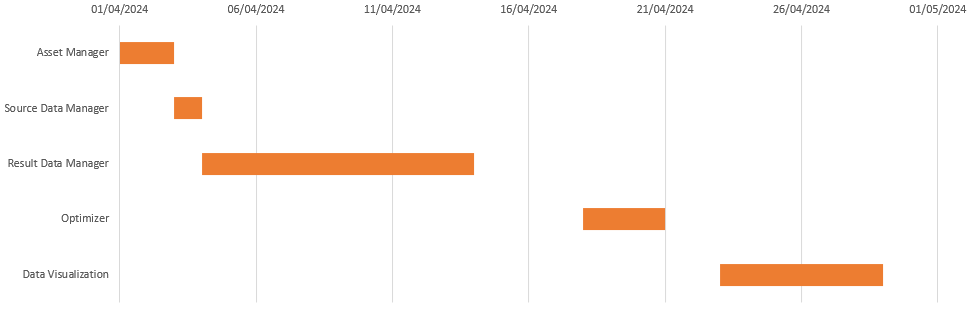
\includegraphics[width=1\textwidth]{Resources/1-Sprint/Gantt-Chart-Optimal.png}
  \caption{Optimal Gantt Chart}
  \label{fig:OptGanttChart}
\end{figure}

\begin{figure}[H]
  \centering
  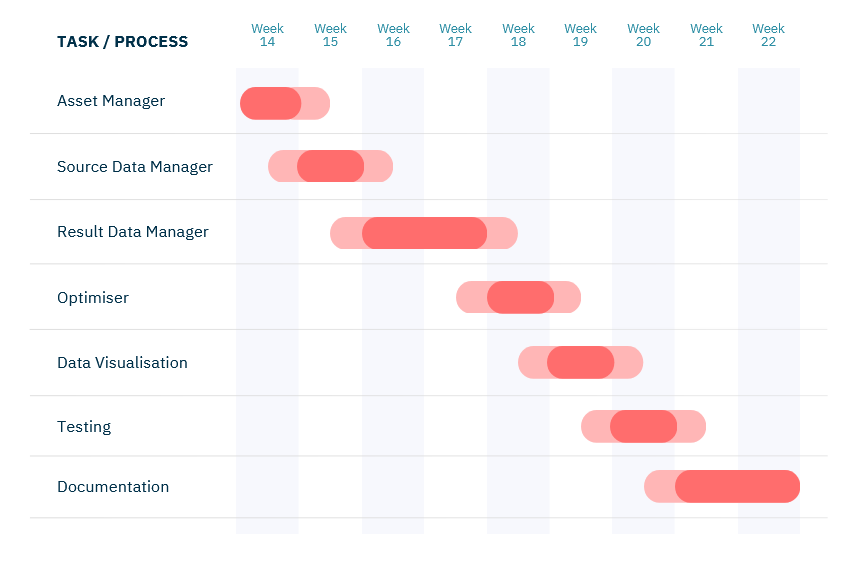
\includegraphics[width=1\textwidth]{Resources/1-Sprint/Gantt-Chart-Realistic.png}
  \caption{Realistic Gantt Chart}
  \label{fig:RealGanttChart}
\end{figure}
\clearpage





\section{Sprint 2}
%Planning
\subsection*{Planning}
\begin{figure}[H]
  \centering
  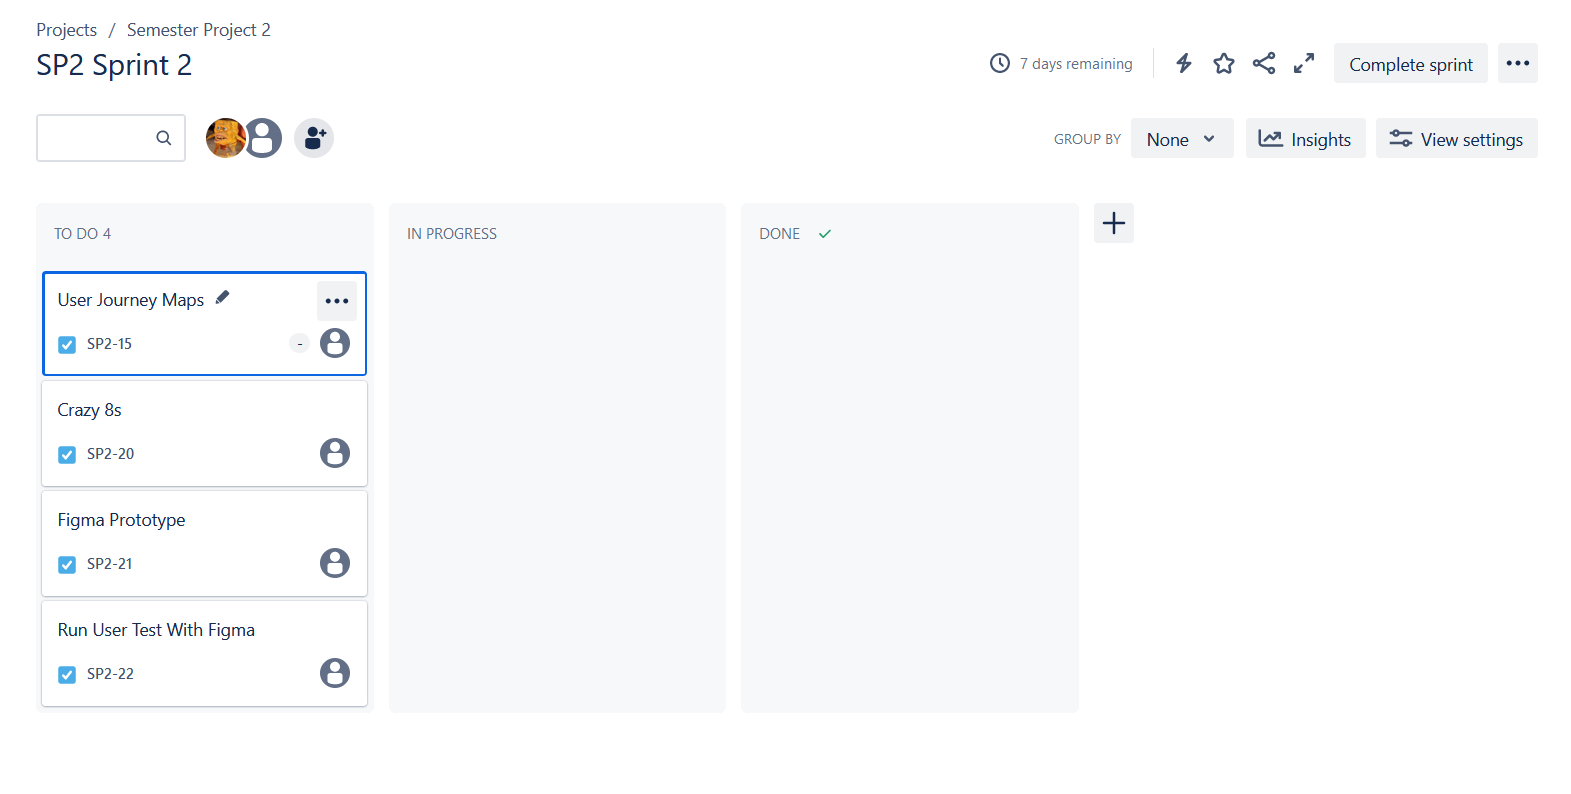
\includegraphics[width=1\textwidth]{Resources/2-Sprint/Planning/Sprint2_Planning_Package.png}
  \caption{Sprint 2 Planning Package}
  \label{fig:S2Planning}
\end{figure}

%Daily Scrum
\subsection*{Daily Scrum 02/04/2024}

\begin{itemize}
    \item The team completed 2 out of 4 issues.
    \item 2 issues are currently in progress, one of which is very close to being finished and the other one is expected to be finished by the end of the week.
\end{itemize}

\subsection*{Roadblocks}
\begin{itemize}
    \item The team faced a few conflicting ideas and a wrong understanding of how the Result Data Manager and Asset Manager components are supposed to look like. They were solved through an online Discord meeting.
    \item Some team members are still on holidays, which makes organising work a bit harder.
\end{itemize}

\subsection*{Plans for the rest of the Sprint}
\begin{itemize}
    \item Polish the Figma prototype made.
    \item Get feedback on the Figma prototype.
    \item Begin discussion about starting the development phase.
\end{itemize}

\subsection*{Metrics and Progress}
The team has attached screenshots of the current state of the sprint backlog and the sprint status report to give information about how much work has been done and how much work still needs to be done.

\begin{figure}[H]
  \centering
  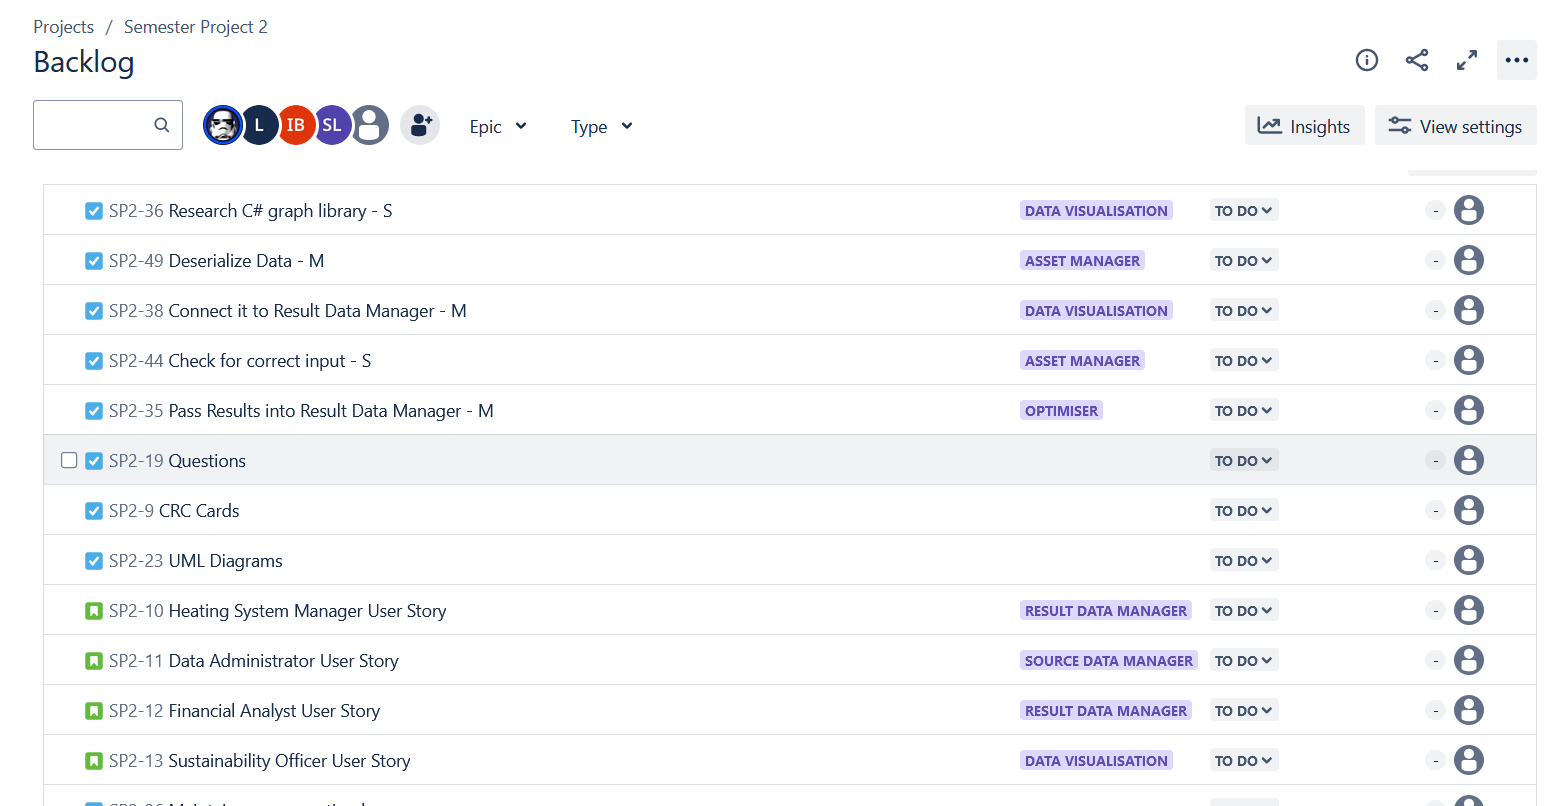
\includegraphics[width=1\textwidth]{Resources/2-Sprint/Daily-Scrum/backlog1.png}
  \caption{Daily Scrum Backlog 1}
  \label{fig:S2Scrum1-image}
\end{figure}

\begin{figure}[H]
  \centering
  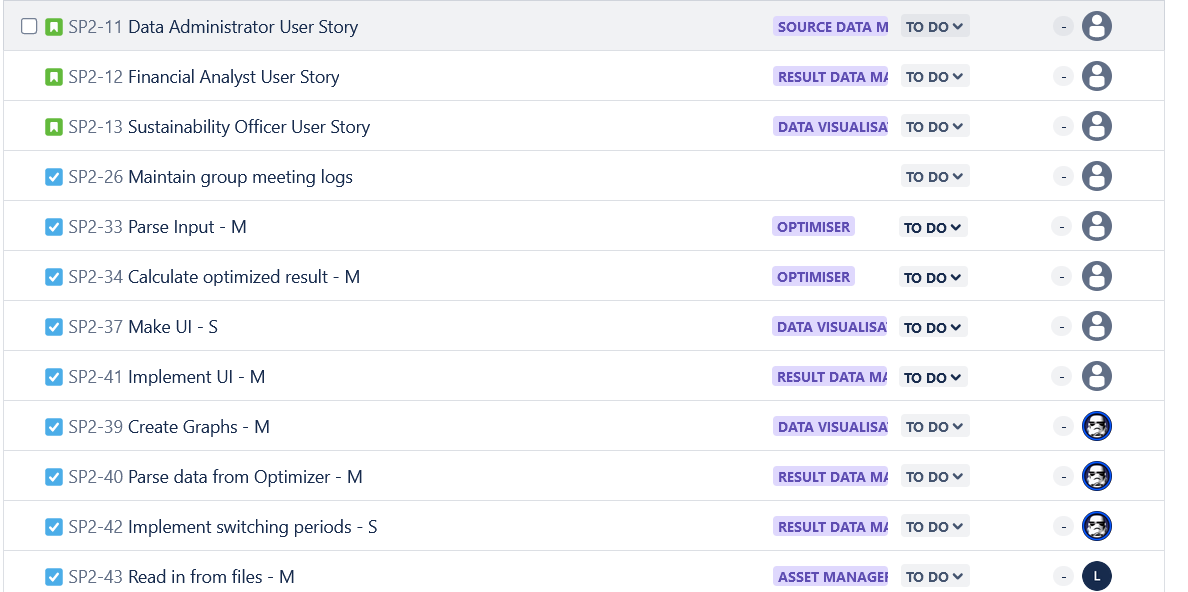
\includegraphics[width=1\textwidth]{Resources/2-Sprint/Daily-Scrum/backlog2.png}
  \caption{Daily Scrum Backlog 2}
  \label{fig:S2Scrum2-image}
\end{figure}

\begin{figure}[H]
  \centering
  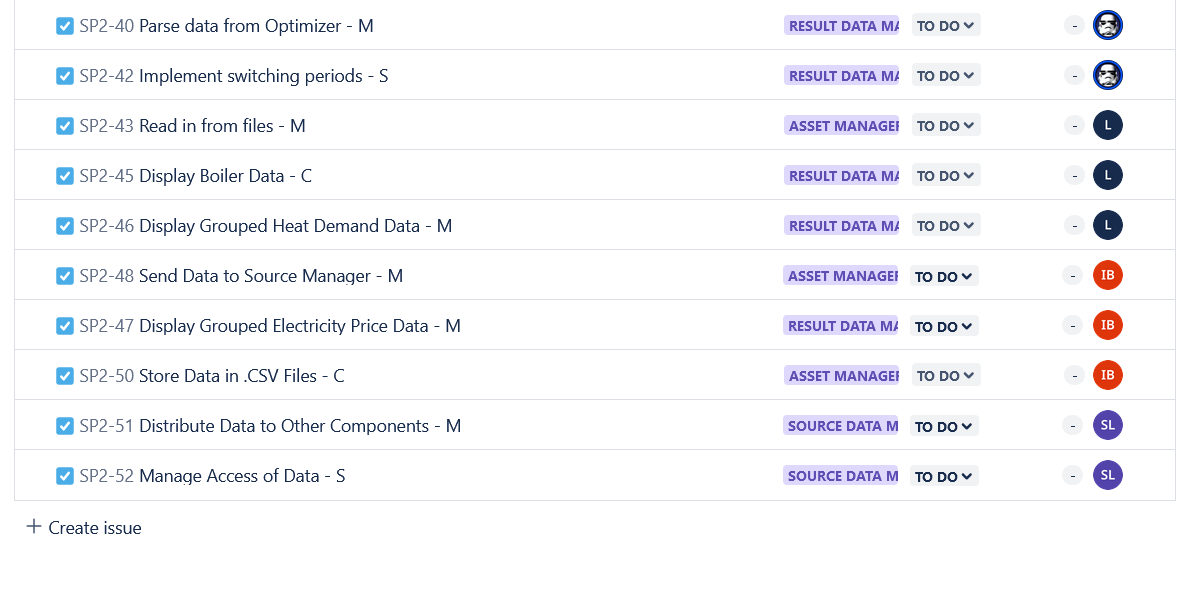
\includegraphics[width=1\textwidth]{Resources/2-Sprint/Daily-Scrum/backlog3.png}
  \caption{Daily Scrum Backlog 3}
  \label{fig:S2Scrum3-image}
\end{figure}

%Retrospective

\subsection*{Sprint Review}

\subsection*{What went well}
\begin{itemize}
    \item Remote meeting to re-align on the project direction
    \item All sprint tasks done despite remote work due to the Easter holidays
    \item Remote communication
    \item Willingness to pivot, make changes to the project
\end{itemize}

\subsection*{What to improve}
\begin{itemize}
    \item Spend more time on understanding the project requirements -- the team had a wrong idea of what the Result Data Manager, Asset Manager and Source Data Manager should consist of which created a setback and meant some of the plans for the project need to be remade, such as the tasks on Jira
    \item Pay attention to time zones when doing remote work -- the time zone difference created a minor issue during one of the team's remote meetings
    \item Plan out and divide work more carefully to avoid misunderstandings and vagueness
\end{itemize}

\subsection*{What the team aims to improve in the next Sprint}
\begin{itemize}
    \item Align the project with the requirements
    \item Remove vagueness from the project direction
    \item Remove vagueness from tasks for each team member
\end{itemize}
\clearpage






\section{Sprint 3}
%Planning
\subsection*{Planning}
The team's goal for this sprint is to be ready for the Midterm Evaluation that is to happen on
Wednesday the 17th of March. The team has planned out to work on the 3 required components:
Result Data Manager, Asset Manager and Source Data Manager. The components will be created in
Asp.Net using Razor Pages and only the boiler configuration for the first iteration will be supported
by the app created. The components will be developed throughout the week depending on the time
of each individual developer . Only one team member was missing during the Sprint 3 Planning
Meeting, and he will be informed of everything discussed through online matters. The only issue that
made the planning process harder was the Jira backlog being outdated due to the product vision
changes. This will be fixed in a future sprint.

\begin{figure}[H]
  \centering
  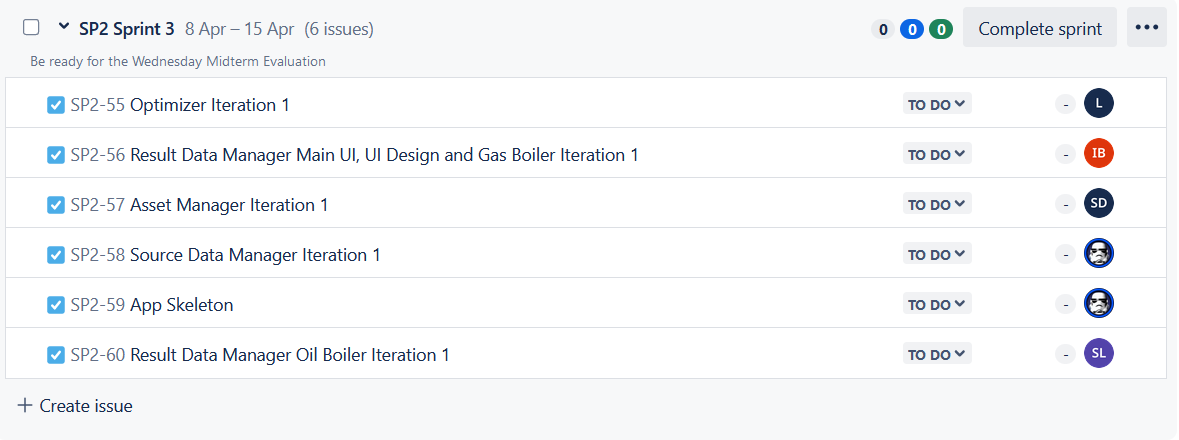
\includegraphics[width=1\textwidth]{Resources/3-Sprint/Planning/Sprint3Planning.png}
  \caption{Sprint 3 Planning}
  \label{fig:S3Planning-image}
\end{figure}
\clearpage

%Scrum
\subsection*{Daily Scrum 16/04/2024}
\subsection*{Team Update}
\begin{itemize}
    \item The team completed 6 out of 6 issues.
    \item The goal for the sprint of being ready for the first iteration presentation has been met.
\end{itemize}

\subsection*{Roadblocks}
\begin{itemize}
    \item Most of the development did not see any roadblocks due to deliberate planning done beforehand.
    \item Team members helped each other to make sure no one is stuck, and the tasks are finished on time.
\end{itemize}

\subsection*{Plans for the Next Sprint}
\begin{itemize}
    \item Fix bugs.
    \item Continue development.
\end{itemize}

\subsection*{Metrics and Progress}
The team has attached screenshots of the current state of the sprint backlog and the sprint status report to give information about how much work has been done and how much work still needs to be done.

\begin{figure}[H]
  \centering
  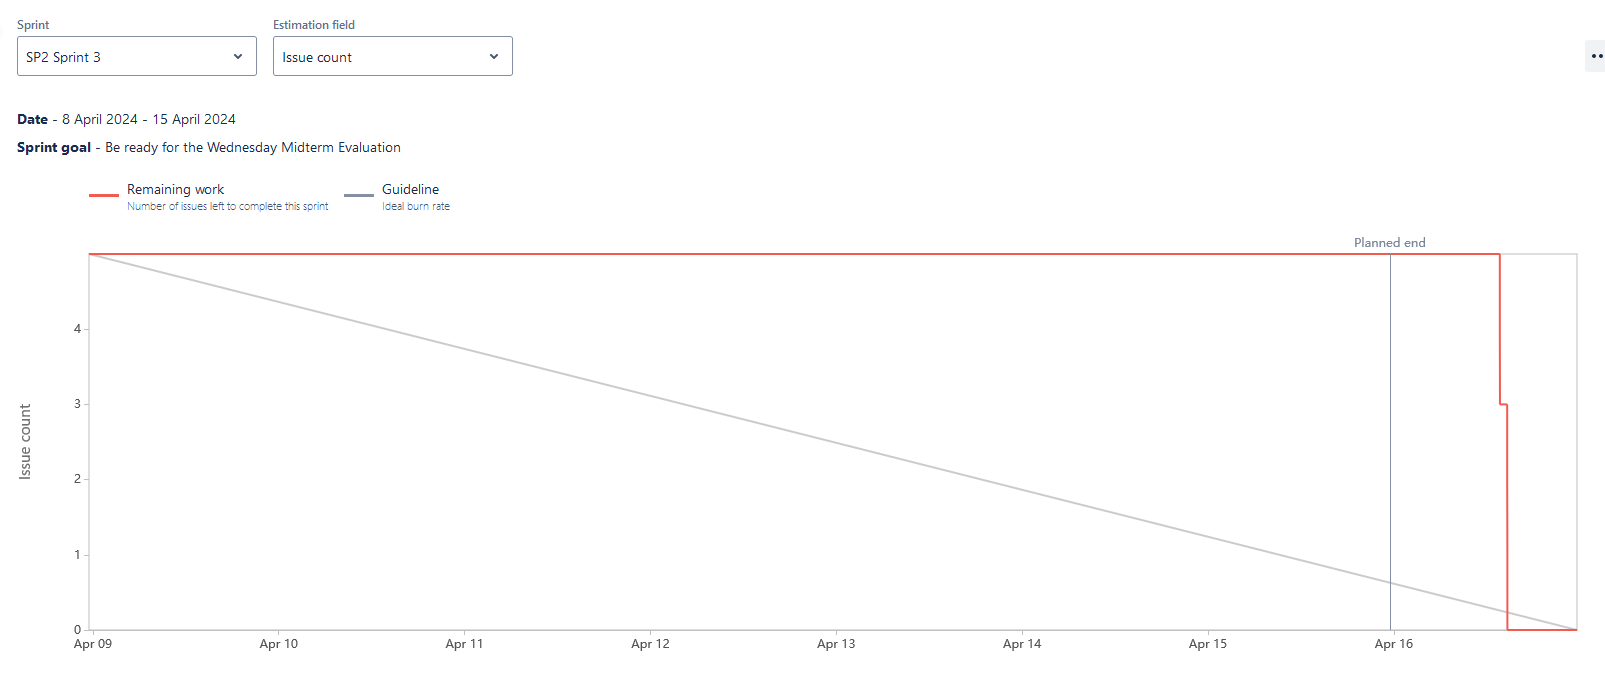
\includegraphics[width=1\textwidth]{Resources/3-Sprint/Daily-Scrum/burndownchart_sprint3.png}
  \caption{Daily Scrum Burndown Chart}
  \label{fig:S3Scrum2-image}
\end{figure}

\begin{figure}[H]
  \centering
  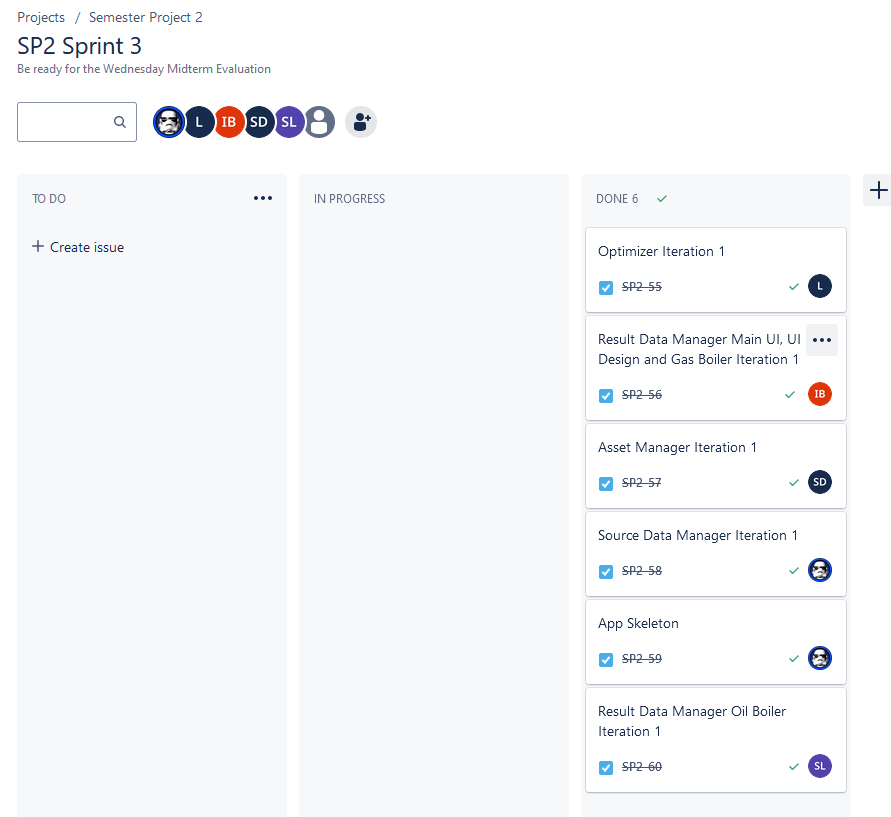
\includegraphics[width=1\textwidth]{Resources/3-Sprint/Daily-Scrum/backlog_sprint3.png}
  \caption{Daily Scrum Backlog}
  \label{fig:S3Scrum1-image}
\end{figure}

\clearpage

%Review

\subsection*{Sprint Review}
\textbf{Project:} Semester Project Group 11 \\
\textbf{Sprint Duration:} April 9 - April 23, 2024 \\
\textbf{Team Members:} Kacper Grzyb \and Sebestyen Deak \and Ignad Bozhinov \and Leonardo Gianola \and Levente Sohar\\
\textbf{Stakeholders:} Sadok Ben Yahia

\subsection*{1. Sprint Goals and Outcomes}
During this sprint, we aimed to iterate our plans for the optimizer program and make a working prototype for the presentation.

\begin{itemize}
    \item \textbf{Goal 1:} Optimizer iteration 1\\
    \textbf{Status:} Completed. The optimizer (for now) looks at the heat demands and if it's below the gas boiler capacity, it only uses that. If exceeded, the other boiler turns on.
    \item \textbf{Goal 2:} UI, UI Design and Gas Boiler Iteration 1\\
    \textbf{Status:} Completed. The app skeleton has been created using Bootstrap for better UX.
    \item \textbf{Goal 3:} Asset Manager Iteration 1\\
    \textbf{Status:} Completed. Created classes for all the boilers, both for iteration 1 and 2.
    \item \textbf{Goal 4:} Source Data Manager Iteration 1\\
    \textbf{Status:} Completed - with minor issue. The Source Data Manager reads in the data from CSV files and creates objects from it. The only issue we have with it is that since Apple's MacOS uses a different DateTime format than Windows, it throws an exception for some of the dates.
    \item \textbf{Goal 5:} Result Data Manager Oil Boiler Iteration 1\\
    \textbf{Status:} Completed.
\end{itemize}

\subsection*{2. Completed Work}
We had the midterm presentation during this sprint, so our main focus was on getting the program in a state that can be presented and making the presentation. We focused on not just making the program work, but also making it easily expandable, therefore we have less work to do in the second iteration. For the visual UI, we used Razor pages, and in that Bootstrap. We made all the components work almost flawlessly, and the end result visually remained close to our Figma prototype.
\subsection*{3. Unfinished Work}
Everything we set out to do during this sprint we have accomplished.
\subsection*{4. Quality and Technical Issues}
There remained to be a bug, where Mac devices aren't able to read in all the data from the CSV file, since the OS expects the months to be where the days are in the source data. So after the day exceeds the 13th day, it throws an exception.
\subsection*{5. Team Dynamics and Collaboration}
Work has been mostly divided equally, with everyone doing their part. Communication was clear and to the point. We had weekly meetings for scrum.
\subsection*{6. Processes and Tools}
Jira helps keep track of the backlog and manage the sprint. Razor pages and Bootstrap have been used for UI. We sometimes looked back at our Figma prototype for reference.
\subsection*{7. Stakeholder Feedback}
After our midterm presentation, we got feedback from 2 supervisors, both were supportive of our development methods and the state of the program. The only criticism we got was regarding our presentation style, and we will try to keep that in mind for the next time.
\subsection*{8. Obstacles and Impediments}
We have been able to complete all the goals without any obstacles or impediments.
\subsection*{9. Successes and Wins}
The biggest win for the team was the feedback we got after the presentation both from the supervisors and the other students.
\subsection*{10. Action Items for Improvement}
Setting a hierarchy amongst tasks so no one has to wait for the other to finish.

\hfill 24/04/2024
\clearpage







\section{Sprint 4}
%Planning
\subsection*{Planning}
The team's aim for this sprint is to try and make the final product, since we only have about 4-5 weeks before having to present it in front of the other students and teachers. This means updating the optimizer, and the UI. We also plan on adding graphs which show the given data, in various configurations. We also plan to fix the bug with the Source Data Manager. Two team members were missing during the Sprint 4 Planning Meeting, but we talked about our goals previously and they will be informed of everything discussed through online matters.

\begin{figure}[H]
  \centering
  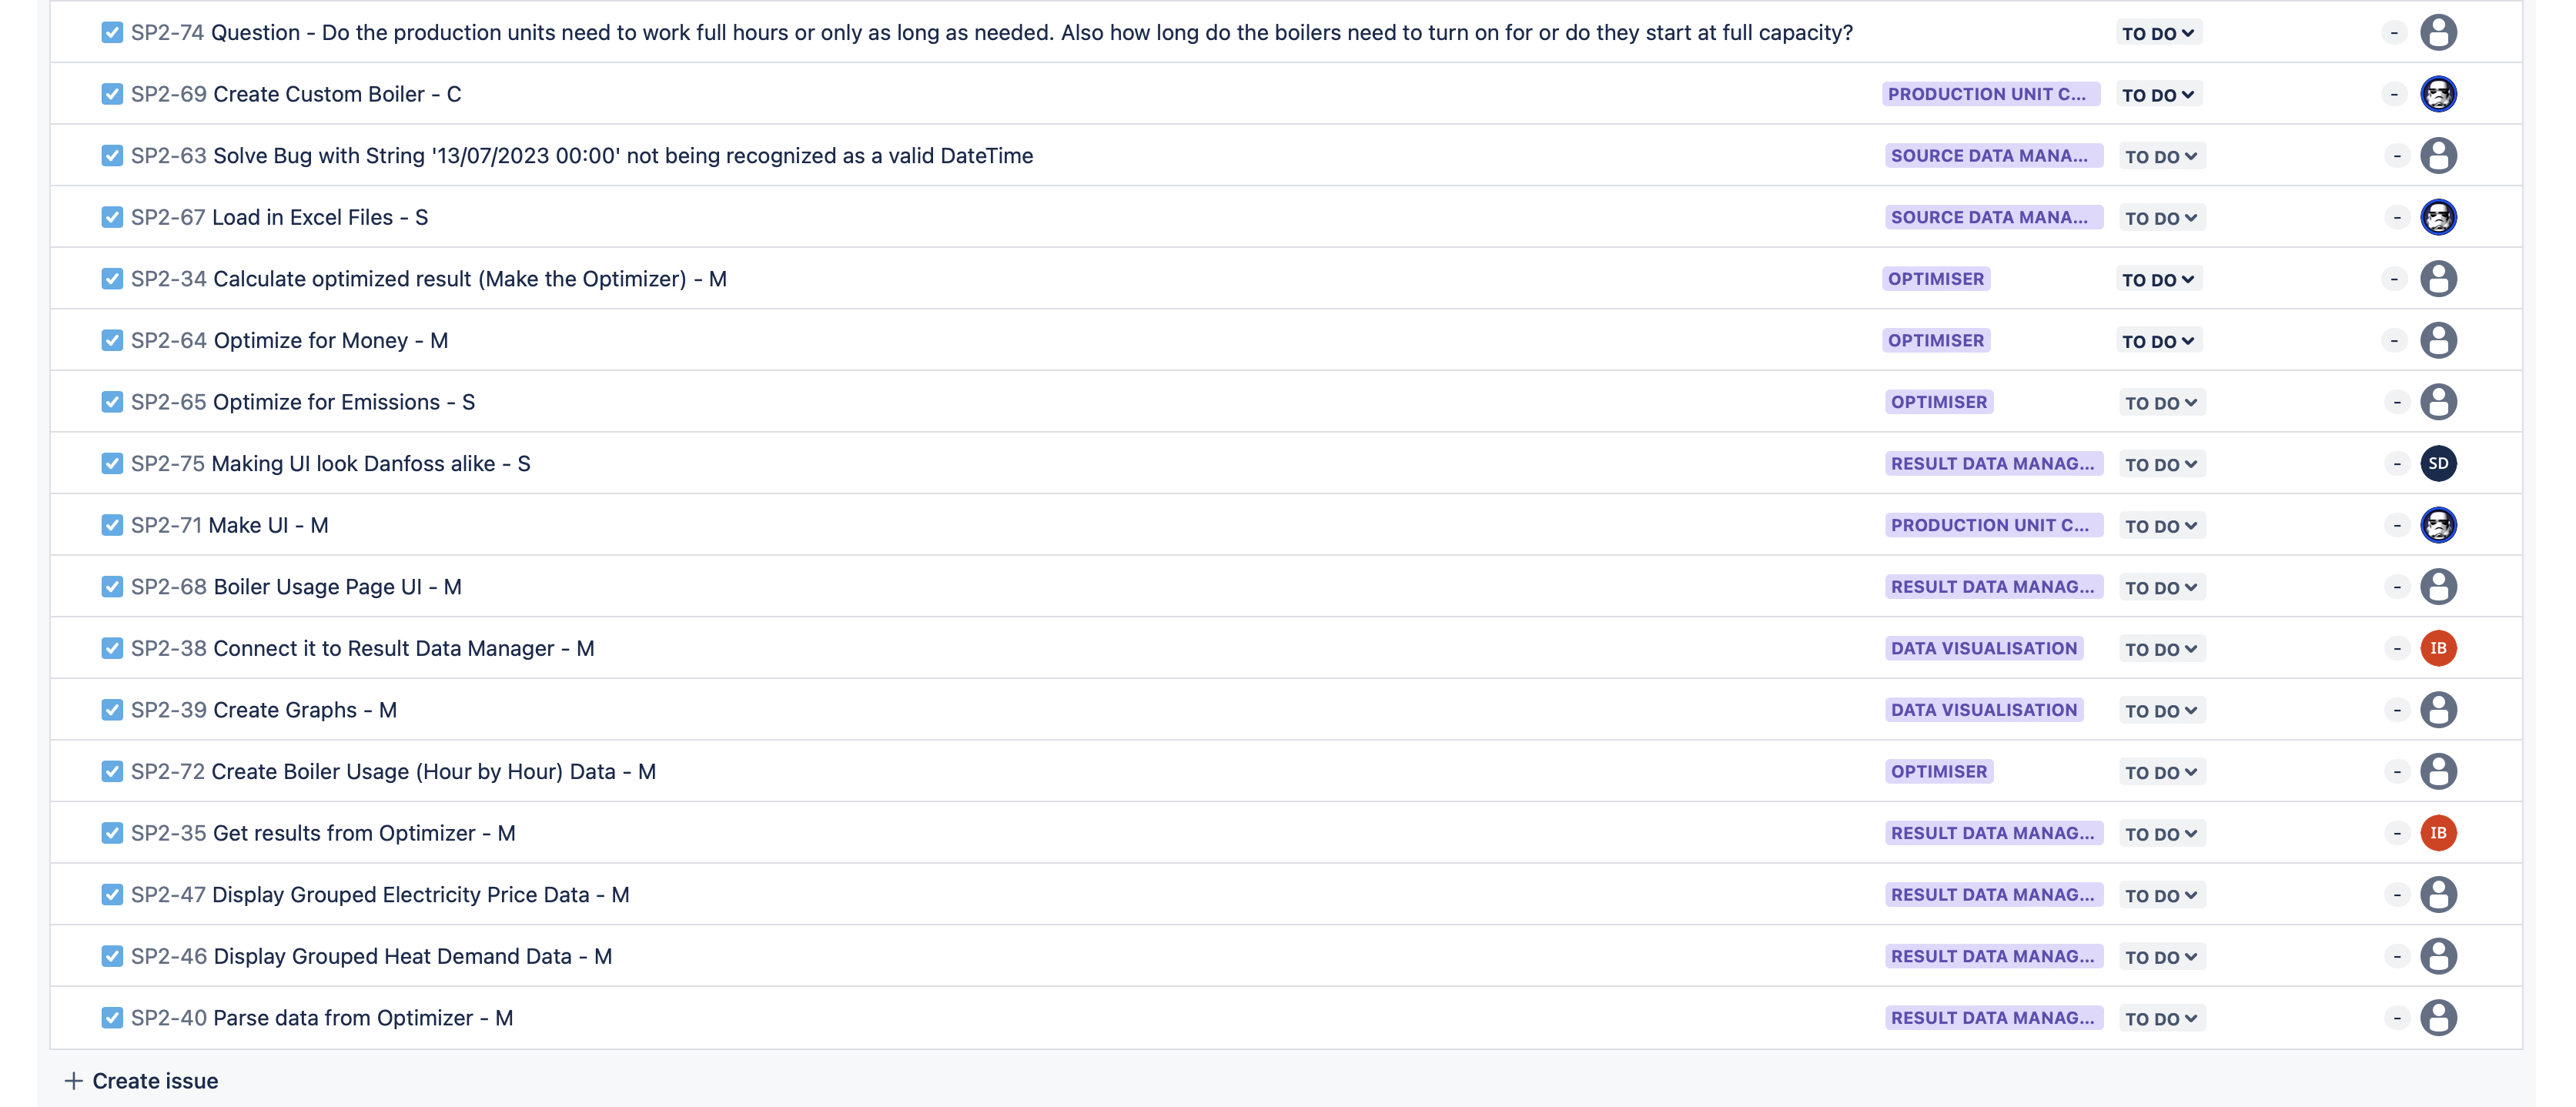
\includegraphics[width=1\textwidth]{Resources/4-Sprint/Planning/Jira.png}
  \caption{Planning Backlog}
  \label{fig:S4Planning-image}
\end{figure}
\clearpage

%Scrum

\subsection*{Daily Scrum 29/04/2024}
\subsection*{Team Update}
\begin{itemize}
    \item The team finished 7 issues and made major progress towards the biggest issue out of 24 issues in the current sprint.
    \item Kacper and Sebestyén will finish work on the optimizer and work on other tasks while Leonardo will continue to work on his neural network optimizer until the end of the sprint. Ignat and Levente are moving on to other tasks.
    \item The goal for the sprint is to complete as many issues as possible.
\end{itemize}

\subsection*{Roadblocks}
\begin{itemize}
    \item The team needed to realign on the approach for the implementation of the optimizer, change the implementation of some of the data structures and get everyone on the same page in the code structure.
    \item Every roadblock was talked about and resolved on this Monday’s meeting.
\end{itemize}

\subsection*{Plans for the Next Sprint}
\begin{itemize}
    \item Continue completing issues from the backlog, while focusing on the must-have features.
    \item Come up with a solution for having multiple optimizers and custom production units.
    \item Make sure all requested features are accounted for in the sprint backlog.
\end{itemize}

\subsection*{Metrics and Progress}
The team has attached screenshots of Jira for progress metrics.

\begin{figure}[H]
  \centering
  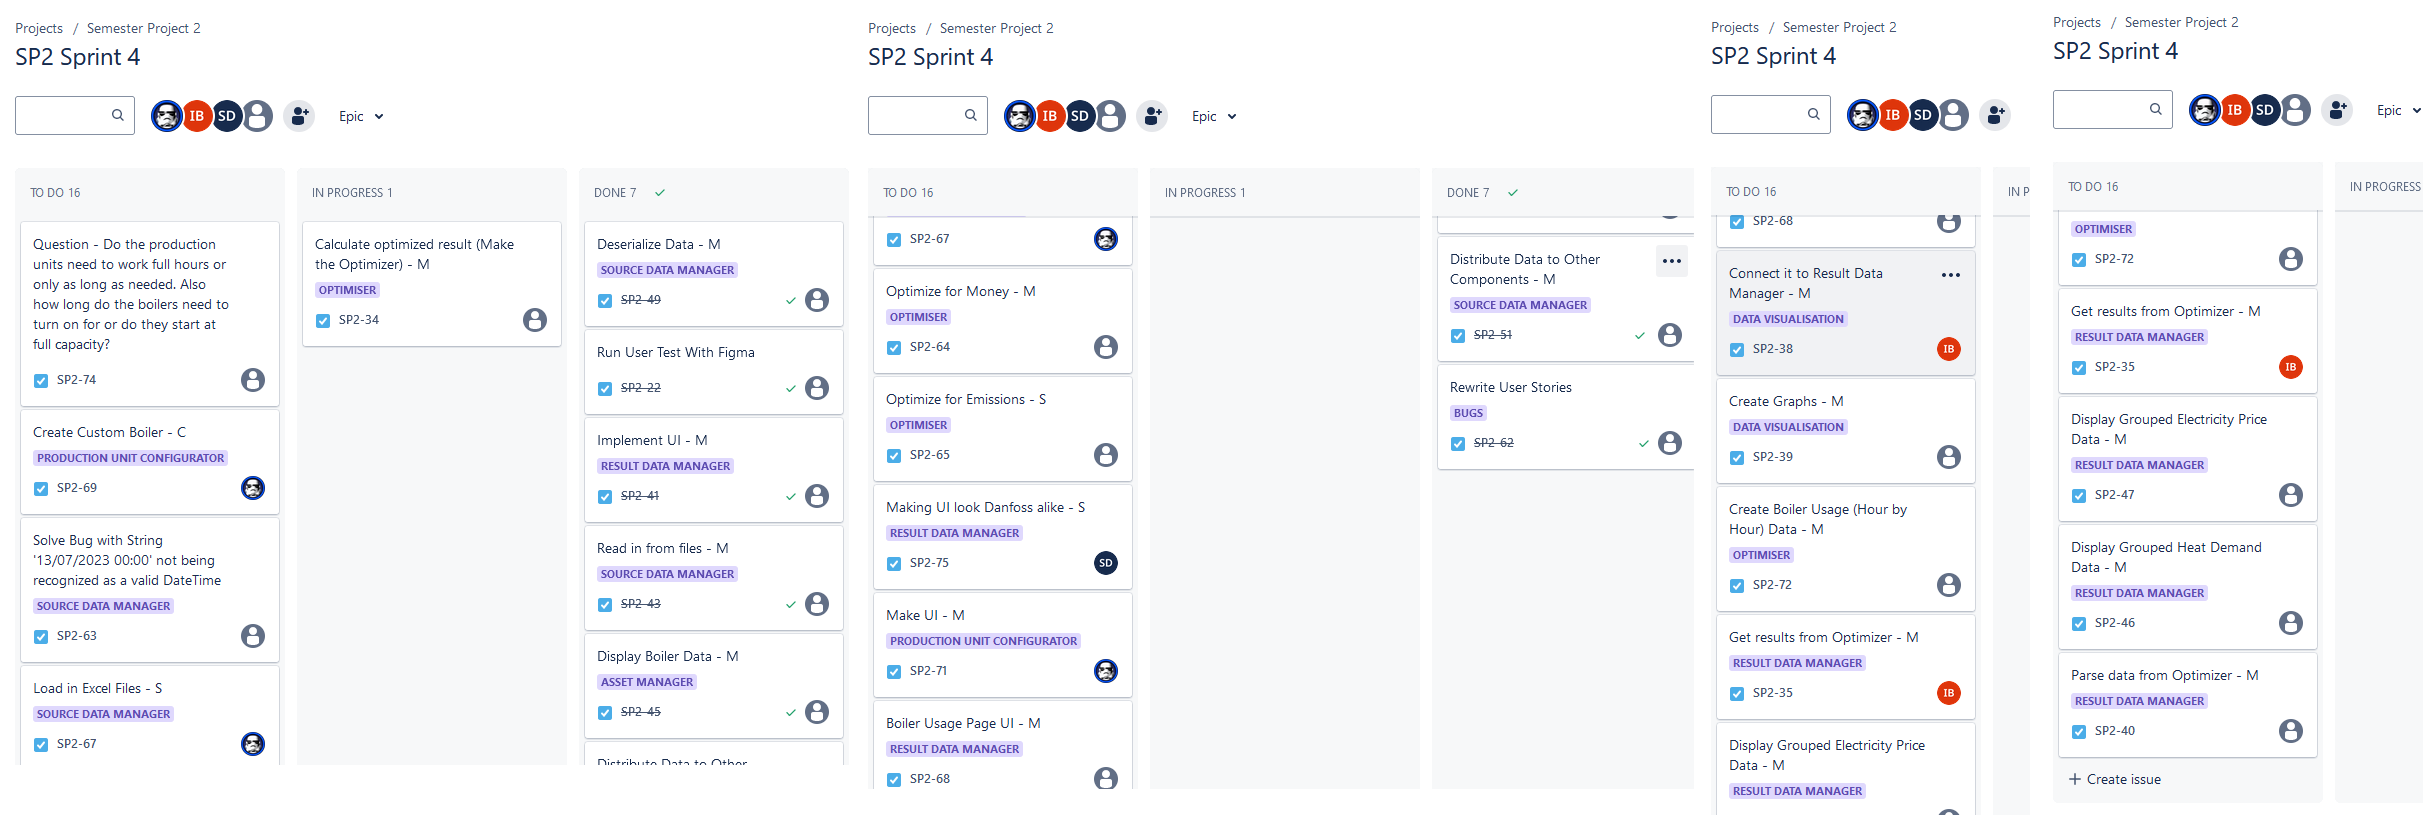
\includegraphics[width=1\textwidth]{Resources/4-Sprint/Daily-Scrum/Backlog.png}
  \caption{Daily Scrum Backlog}
  \label{fig:S4Scrum-image}
\end{figure}
\clearpage

%Review
\subsection*{Sprint Review}
\textbf{Project:} Semester Project Group 11 \\
\textbf{Sprint Duration:} April 23 - May 7, 2024 \\
\textbf{Team Members:} Kacper Grzyb \and Sebestyen Deak \and Ignad Bozhinov \and Leonardo Gianola \and Levente Sohar\\
\textbf{Stakeholders:} Sadok Ben Yahia

\subsection*{1. Sprint Goals and Outcomes}
The goal for this sprint was to start fully developing the program. For this, we added every issue that's a must (according to the MoSCoW breakdown we made) for the minimal viable product. We overshot our capabilities on purpose, so we see what to do, and we will continue working on this in the next sprint as well.
\begin{itemize}
    \item \textbf{Goal 1:} Create Comparable Data\\
    \textbf{Status:} Completed. Created two additional classes based on the Optimizer class, that create scenarios which are not the optimal case, to have something to compare our solution to.
    \item \textbf{Goal 2:} Boiler Usage Data\\
    \textbf{Status:} In Progress. The data of which boiler is running when is created, it needs to be grouped and displayed to the user.
    \item \textbf{Goal 3:} Neural Network Optimizer\\
    \textbf{Status:} In Progress. The program is written for a neural engine to find the optimal solution, it just needs to be trained, and then introduced to the project environment.
    \item \textbf{Goal 4:} Create Graphs\\
    \textbf{Status:} To Do. We plan on displaying the different scenarios for the user next to each other in bar graphs.
    \item \textbf{Goal 5:} Choosing Boilers for the Optimization\\
    \textbf{Status:} To Do. We want the user to be able to choose which boilers they want to use to get the optimized results.
    \item \textbf{Goal 6:} Save to CSV files\\
    \textbf{Status:} To Do.
\end{itemize}

\subsection*{2. Completed Work}
The members of the group are focusing on the upcoming Mathematics Exam, not on the project. The next sprint is planned to be more productive. Still, everyone is moving slowly forward with their to-dos. The only task that has been fully accomplished was requested by our supervisor.
\subsection*{3. Unfinished Work}
Many things, including the Data Visualization, Creating and Choosing boilers.
\subsection*{4. Quality and Technical Issues}
All the bugs from the last sprint have been fixed. There are no known issues at the moment.
\subsection*{5. Team Dynamics and Collaboration}
Work has been mostly divided equally, with everyone doing their part. Communication was clear and to the point. We had weekly meetings for scrum.
\subsection*{6. Processes and Tools}
Jira helps keep track of the backlog and manage the sprint. Razor pages and Bootstrap have been used for UI. We sometimes looked back at our Figma prototype for reference.
\subsection*{7. Stakeholder Feedback}
The feedback of our supervisor has been to provide some reference point for the data that our optimizer gives as the end result. This has been mostly accomplished in this sprint.
\subsection*{8. Obstacles and Impediments}
The pressure of the upcoming math test reflected on the amount of work done.
\subsection*{9. Successes and Wins}
There has not been any outstanding win or success during this sprint.
\subsection*{10. Action Items for Improvement}
Pass the exam with good grades, so all energy can be focused on the project.
\hfill 07/05/2024

\begin{figure}[H]
  \centering
  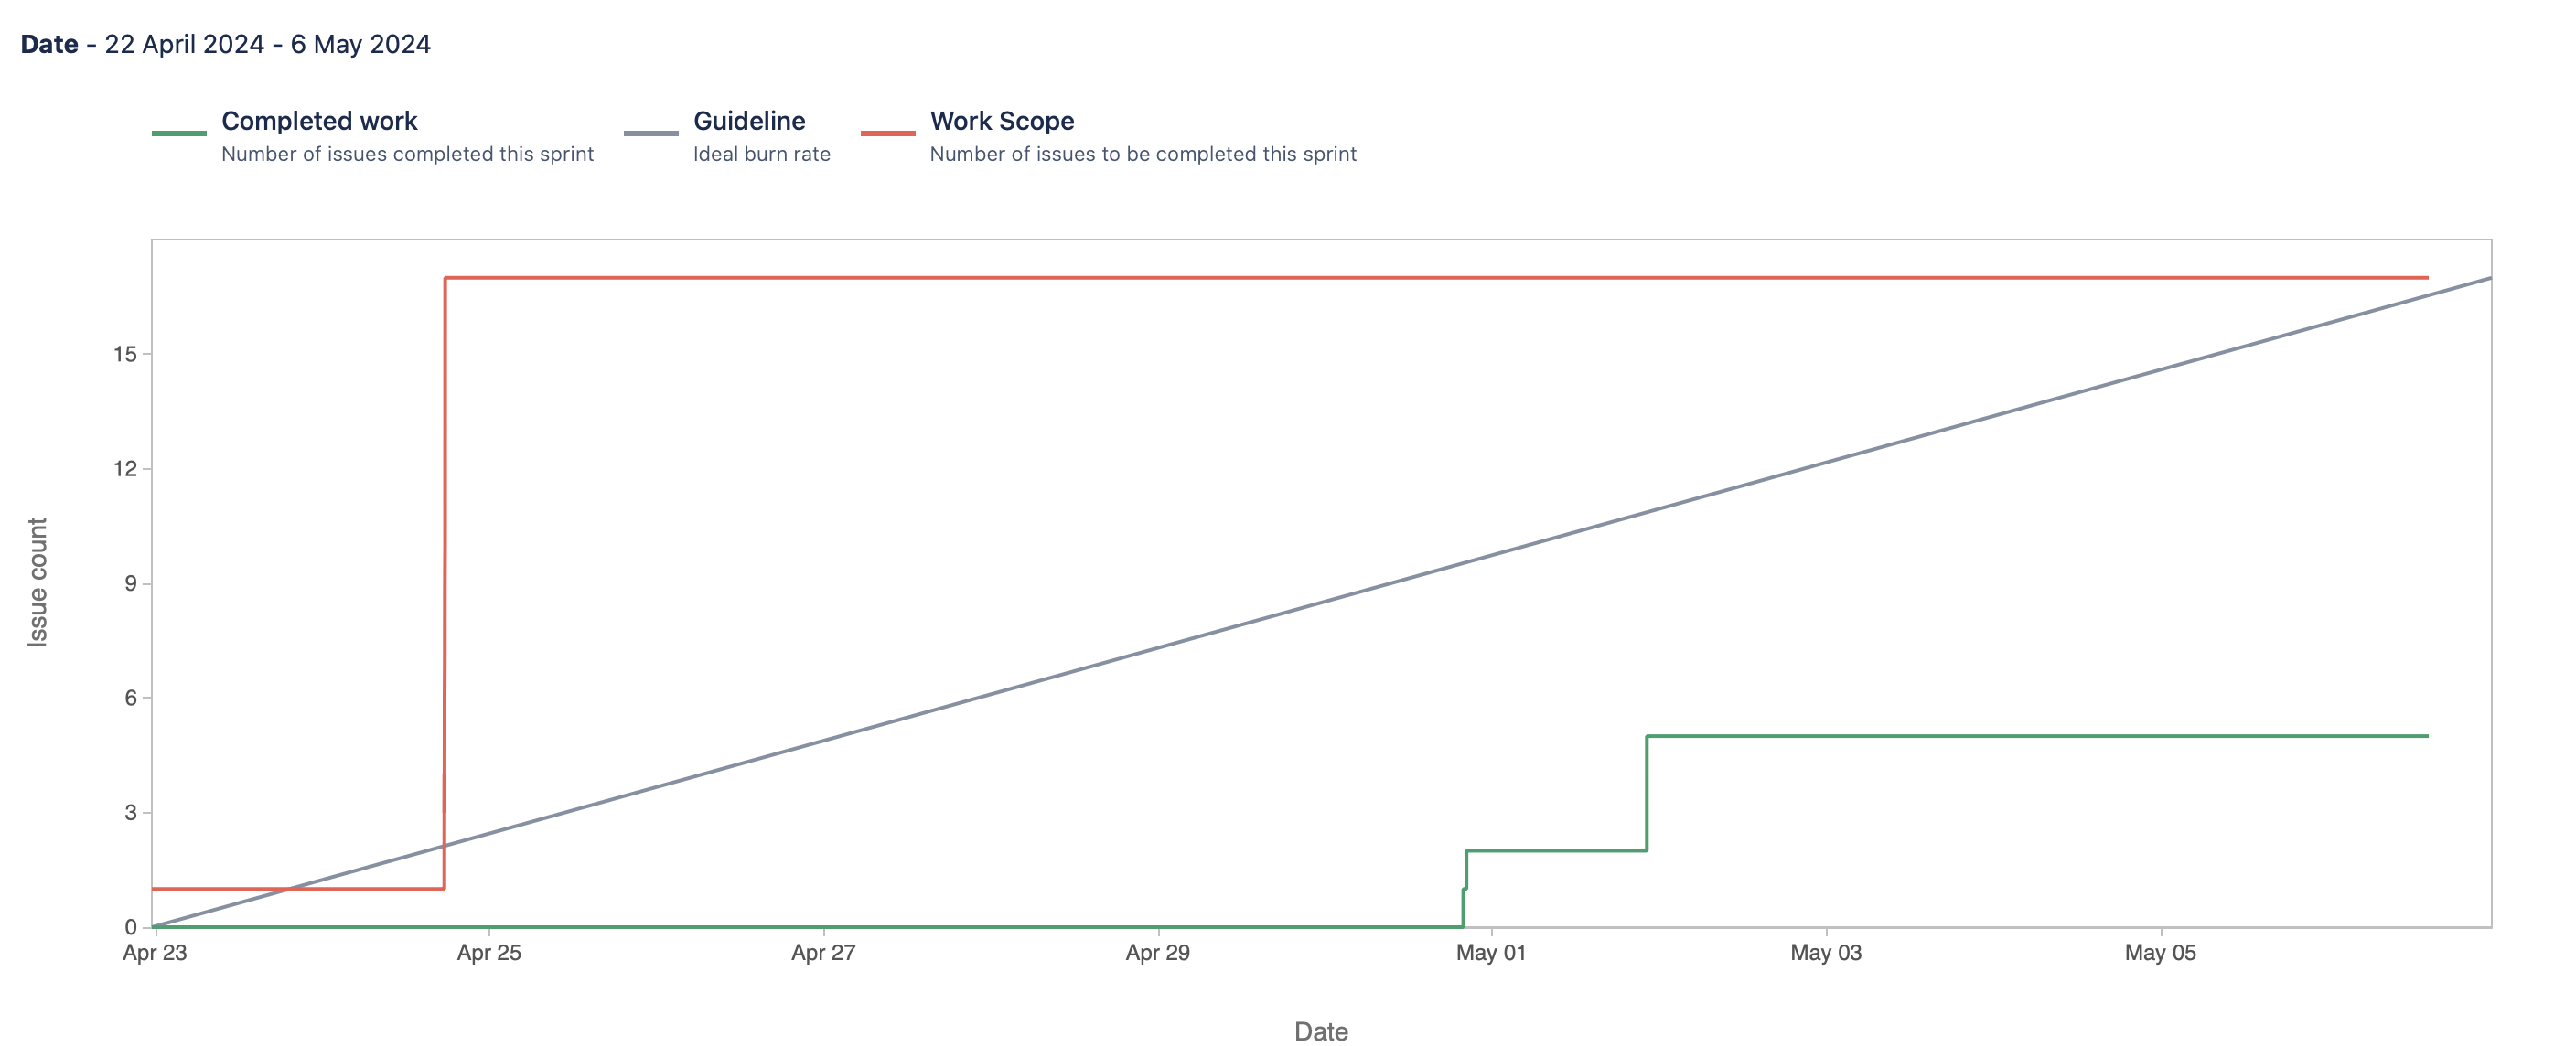
\includegraphics[width=1\textwidth]{Resources/4-Sprint/Review/Burndown.png}
  \caption{Sprint 4 Burnup Report}
  \label{fig:S4Burndown-image}
\end{figure}

\begin{figure}[H]
  \centering
  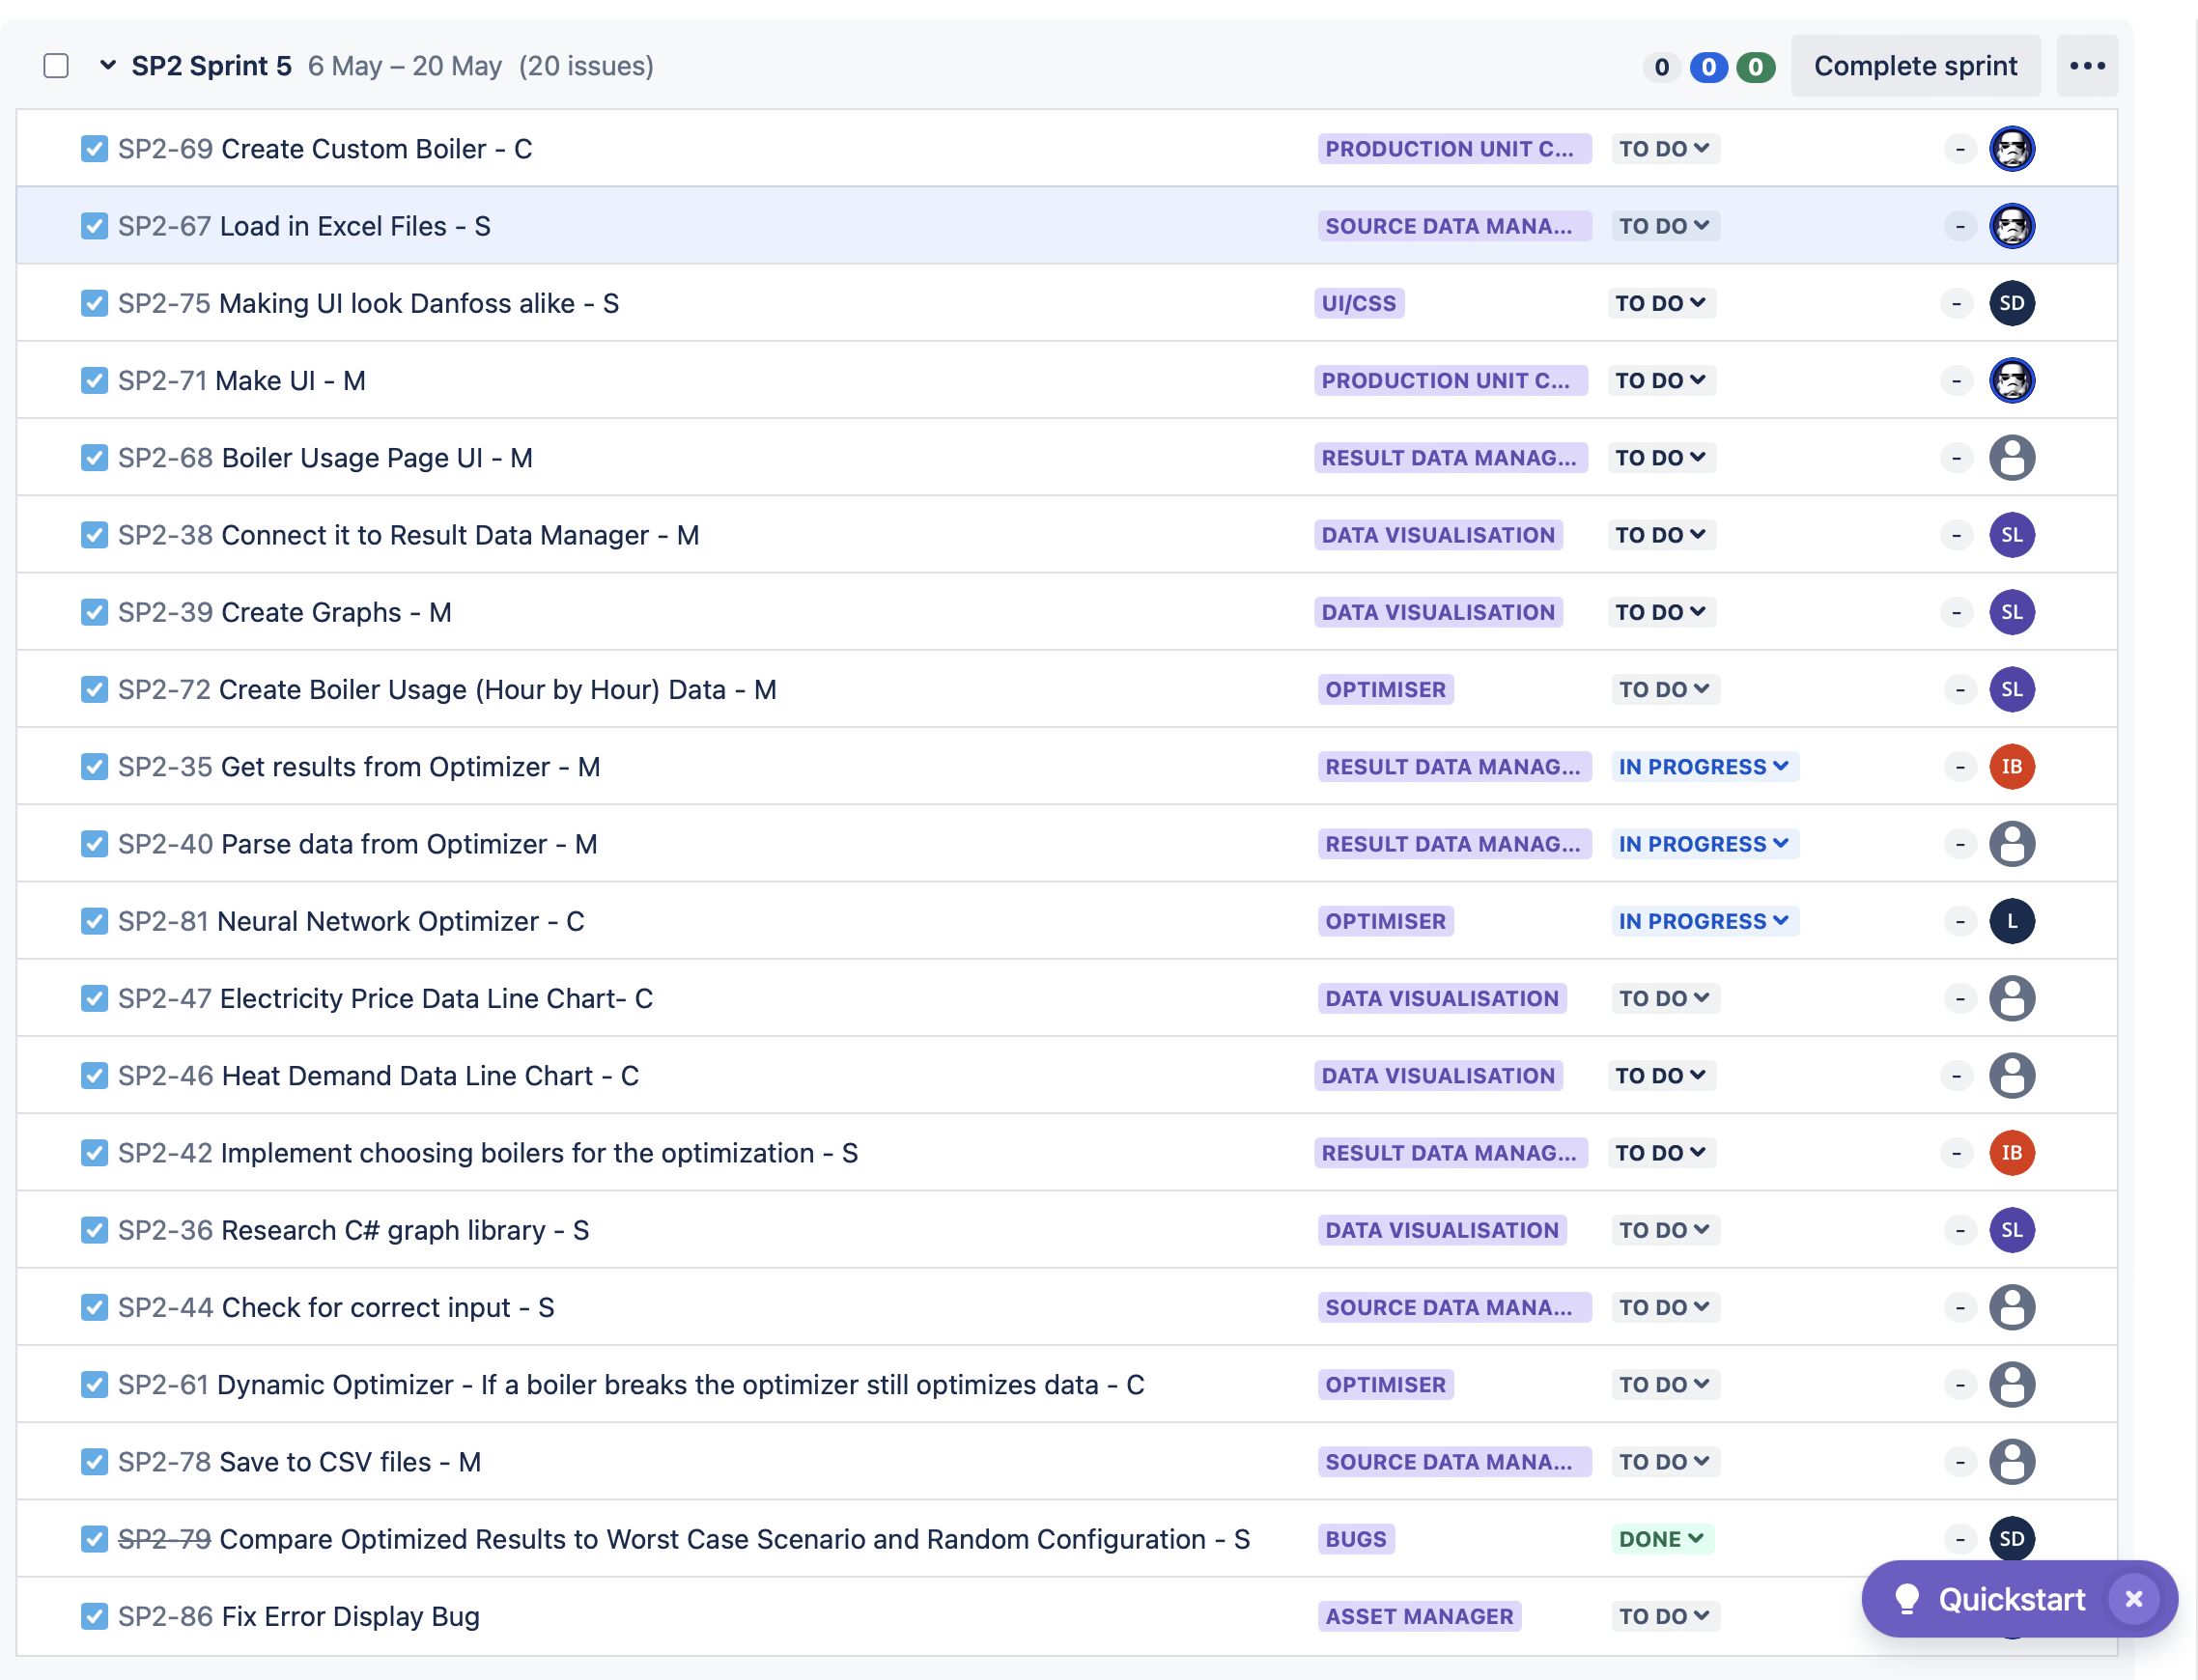
\includegraphics[width=1\textwidth]{Resources/4-Sprint/Review/Issues.png}
  \caption{Sprint 4 Issues}
  \label{fig:S4Issues-image}
\end{figure}
\clearpage







\section {Sprint 5}
%Planning
\subsection*{Planning}
We aim on delivering an almost final version of our product. The Danfoss Demo is going to take place at the end of this Sprint, and we want more than the MVP to be ready by then. We plan on making the Data Visualization with showing the end result and maybe the initial data given in, boiler customization and choosing which one to run for the optimization and a few more smaller things. All members were present on the meeting, and issues have been distributed among us.

\begin{figure}[H]
  \centering
  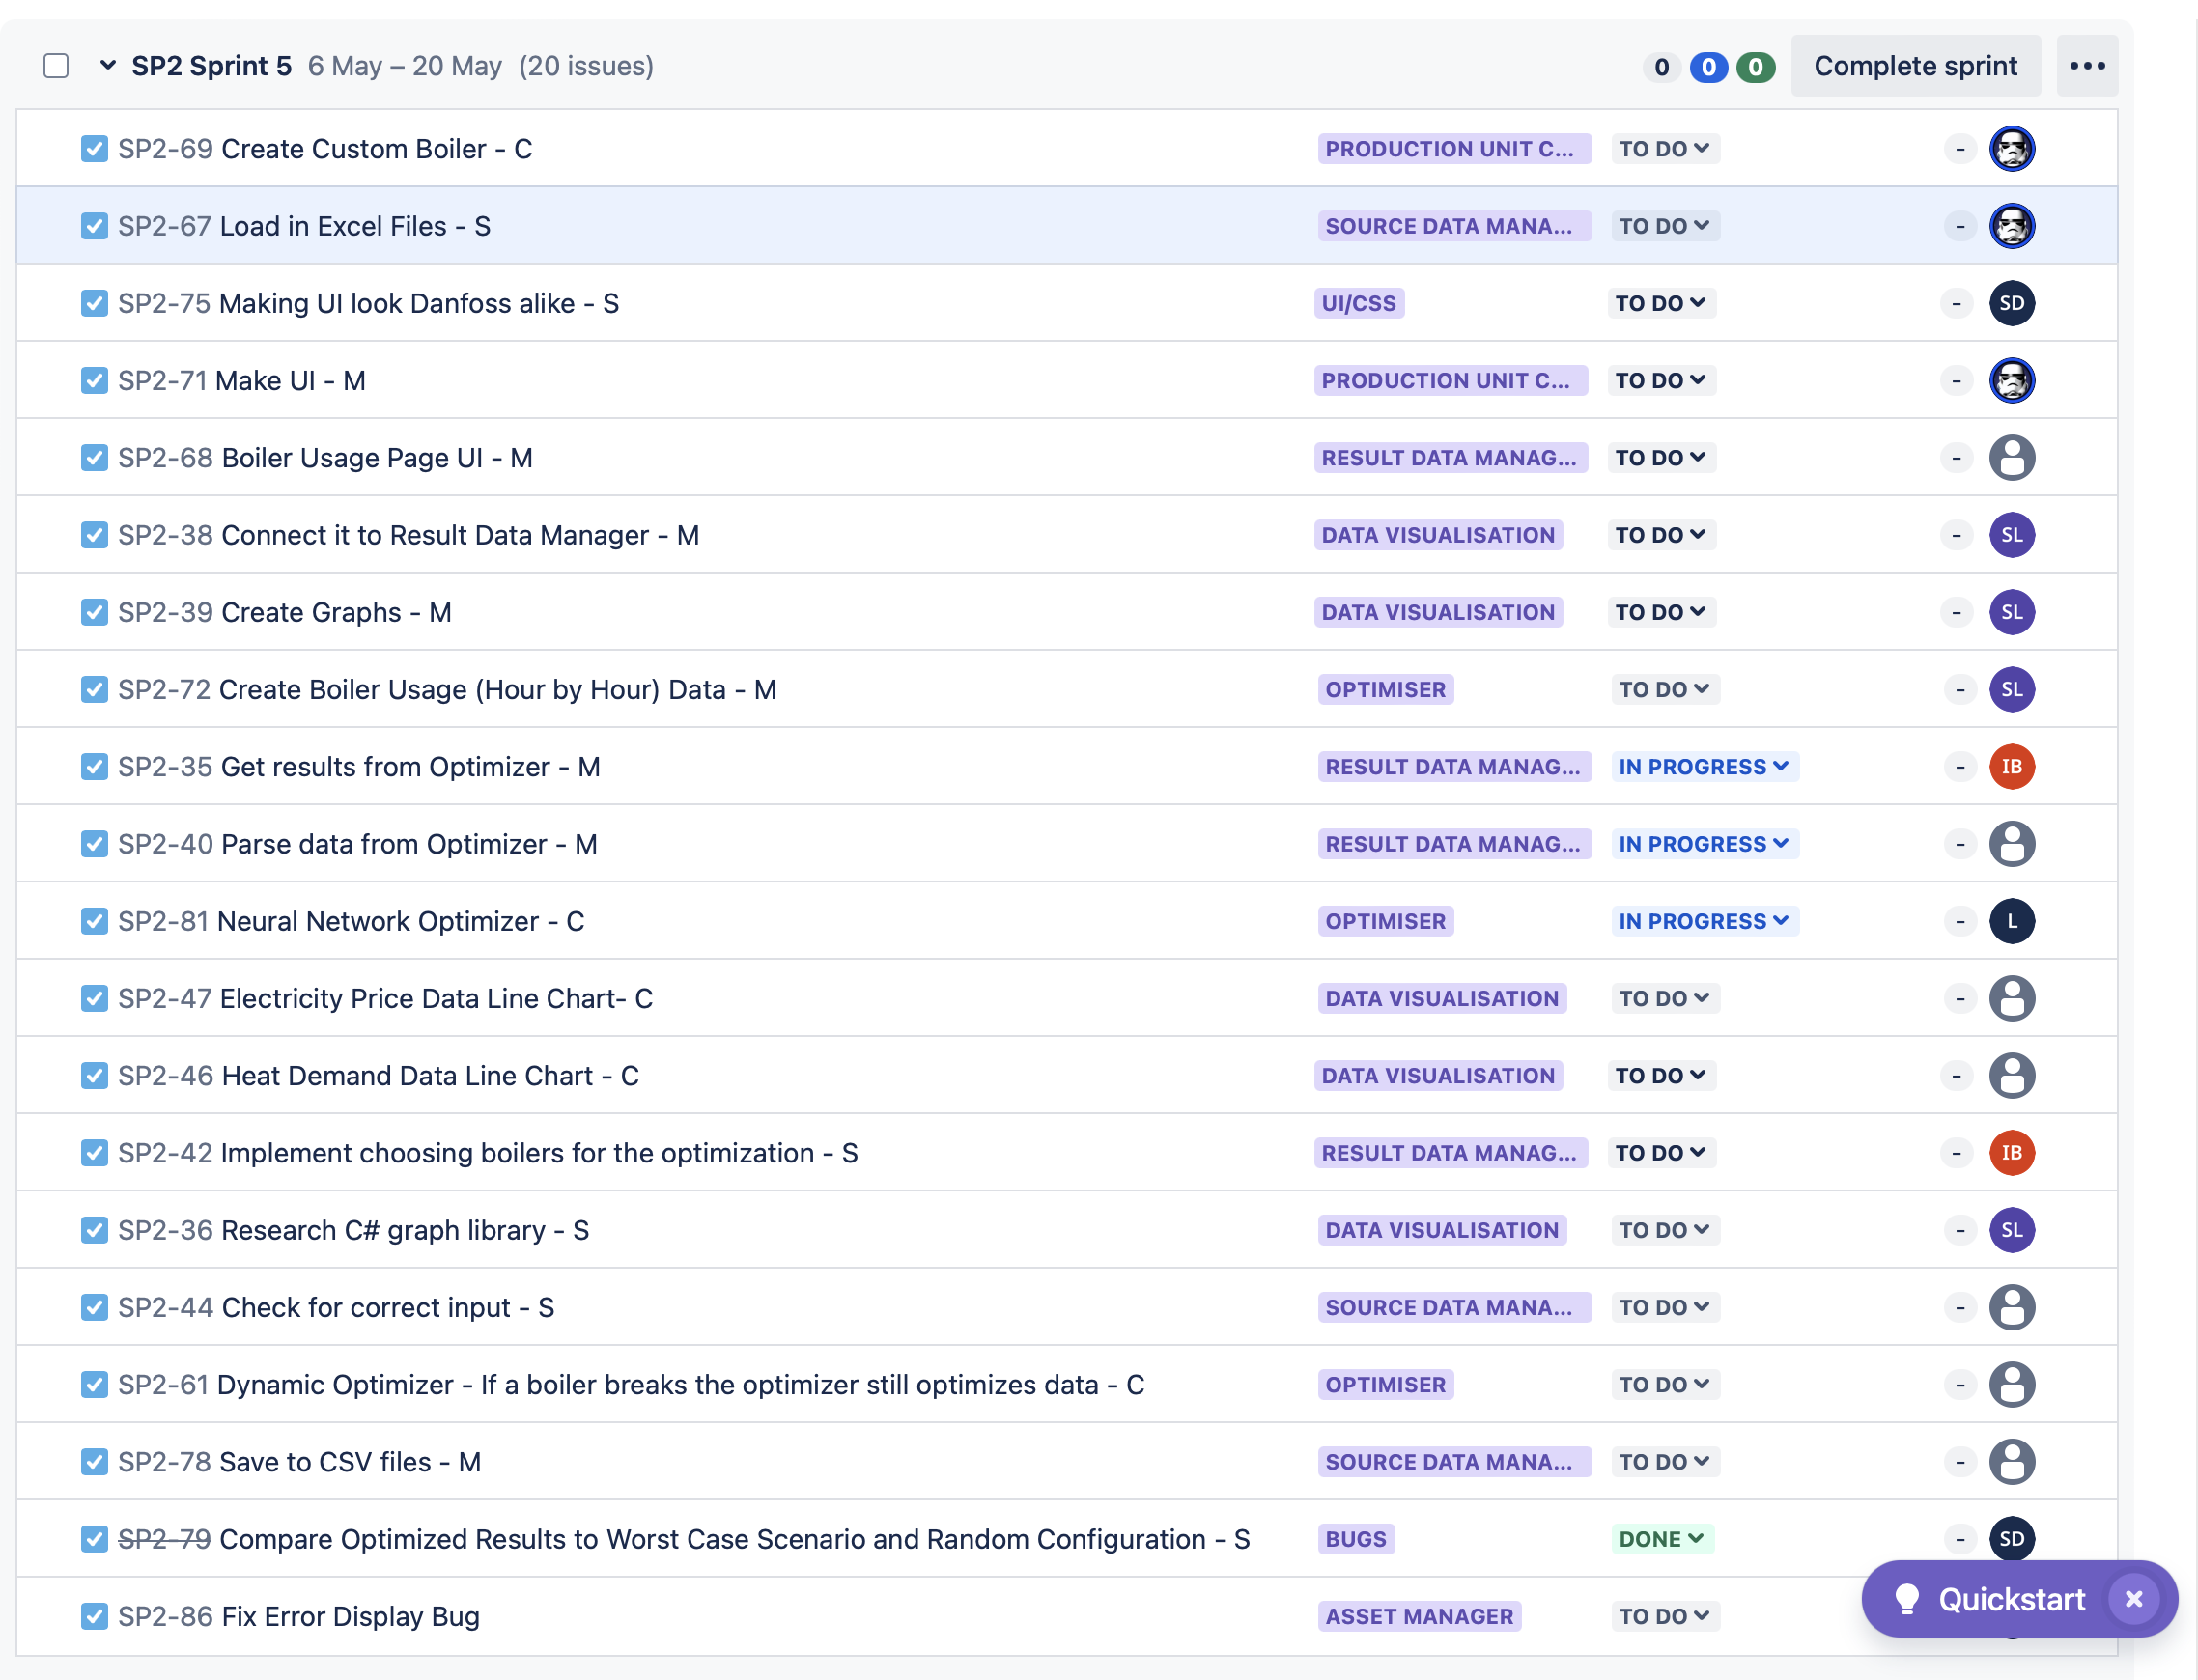
\includegraphics[width=1\textwidth]{Resources/5-Sprint/Planning/Jira.png}
  \caption{Planning Backlog}
  \label{fig:S5Planning-image}
\end{figure}
\clearpage

%Scrum
\subsection*{Daily Scrum 19/05/2024}
\subsection*{Team Update}
\begin{itemize}
    \item The team finished 7 issues and made major progress towards the biggest issue out of the 24 issues in the current sprint.
    \item Leonardo is continuing to work on the Neural Network solution for the optimizer. Levente is making the graphs to show and compare the data from the program. Ignat is finalizing the looks of the pages. Kacper and Sebi are working on being able to read in and to save to different files.
    \item The goal for the sprint is to get as close to the final product as possible for the presentation at the end of this sprint.
\end{itemize}

\subsection*{Roadblocks}
\begin{itemize}
    \item The team was slowed down by the math exam last week.
    \item Every roadblock was talked about and resolved in this meeting.
\end{itemize}

\subsection*{Plans for the Next Sprint}
\begin{itemize}
    \item Because we plan on finishing all the must features next sprint, we plan on polishing any mistakes, and maybe adding a few of the Could features.
    \item Build on the feedback given at the presentation.
    \item Make sure all requested features are accounted for in the sprint backlog.
\end{itemize}

\subsection*{Metrics and Progress}
The team has attached screenshots of Jira for progress metrics.

\begin{figure}[H]
  \centering
  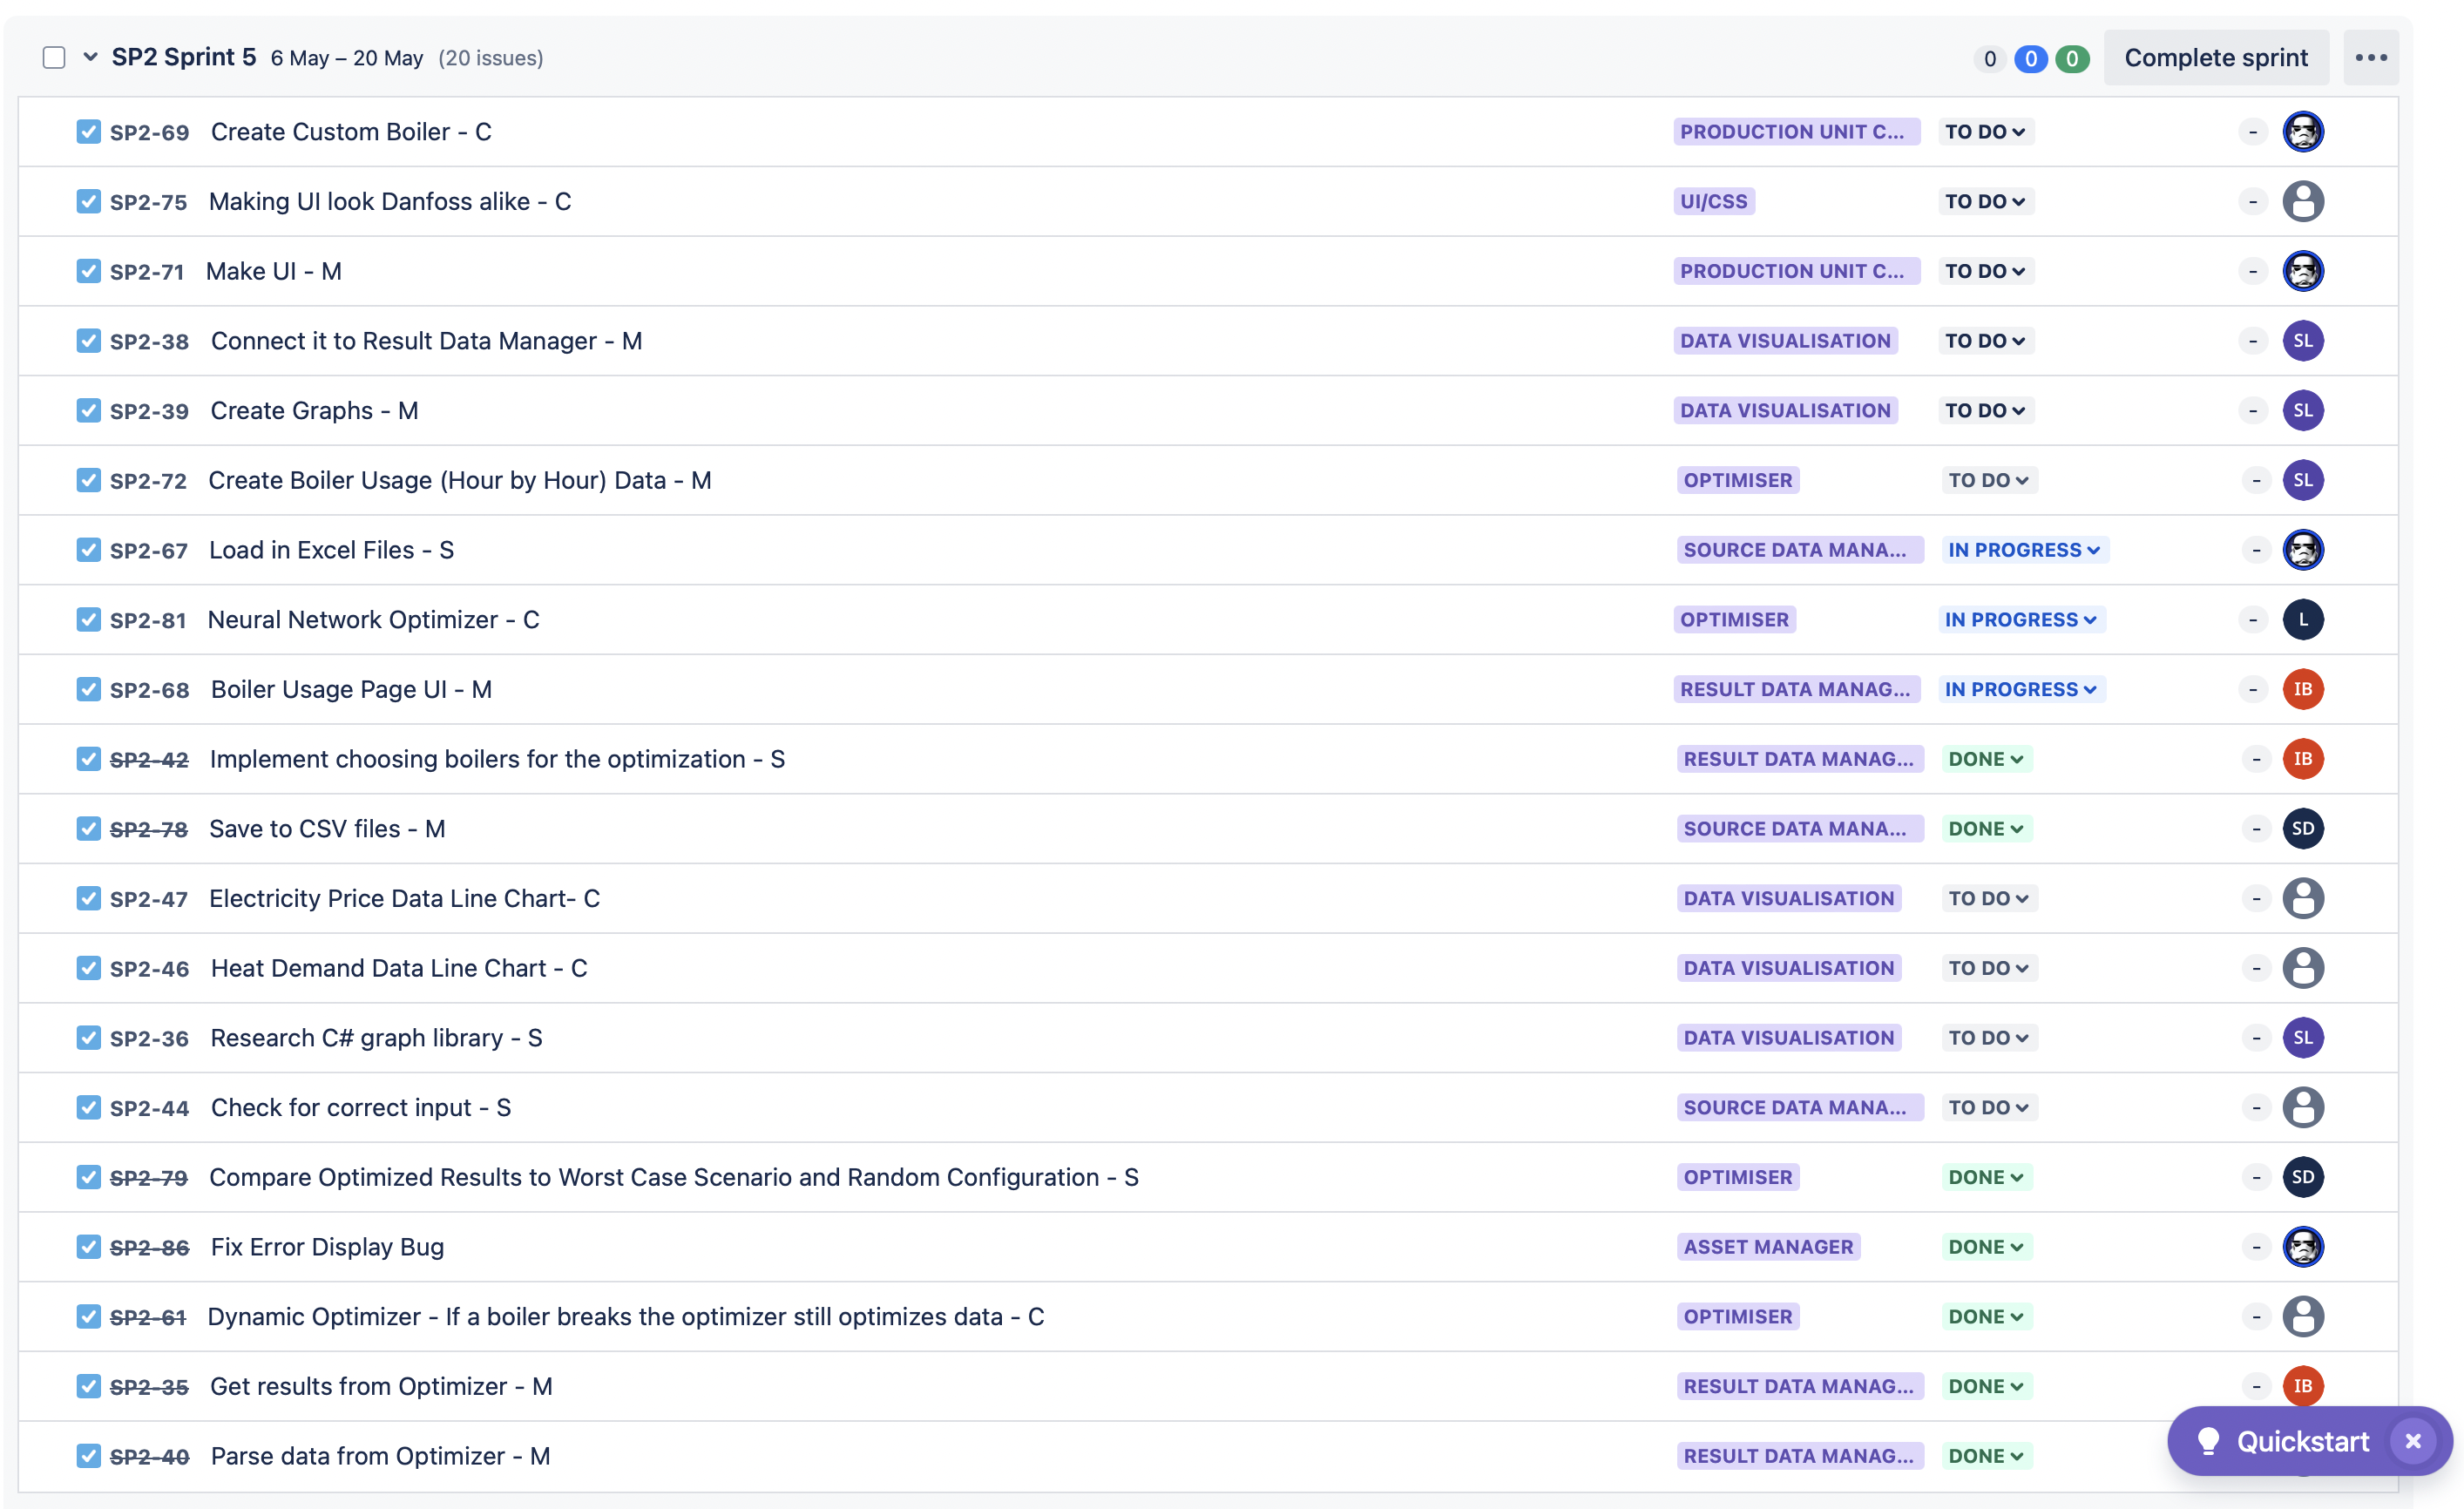
\includegraphics[width=1\textwidth]{Resources/5-Sprint/Daily-Scrum/Jira.png}
  \caption{Daily Scrum Backlog}
  \label{fig:S5Scrum-image}
\end{figure}
\clearpage

%Review
\subsection*{Sprint Review}
\textbf{Project:} Semester Project Group 11 \\
\textbf{Sprint Duration:} May 7 - May 21, 2024 \\
\textbf{Team Members:} Kacper Grzyb \and Sebestyen Deak \and Ignad Bozhinov \and Leonardo Gianola \and Levente Sohar\\
\textbf{Stakeholders:} Sadok Ben Yahia

\subsection*{1. Sprint Goals and Outcomes}
The goal for this sprint was to finish developing the program’s must-have features and polish them to be acceptable for the presentation. We carried on with the remaining tasks from Sprint 4 and continued the development of the full program.
\begin{itemize}
    \item \textbf{Goal 1:} Create Boiler Usage\\
    \textbf{Status:} Completed. Created an additional page inside the program, where the distribution amongst boilers can be viewed, in addition to the saving options.
    \item \textbf{Goal 2:} Create Custom Boiler\\
    \textbf{Status:} Completed. The user of the program can now create a fully customizable boiler.
    \item \textbf{Goal 3:} Neural Network Optimizer\\
    \textbf{Status:} Completed. The program is written for a neural engine to find the optimal solution.
    \item \textbf{Goal 4:} Create Graphs\\
    \textbf{Status:} Completed. All vital and comparable data is displayed for the user to put the optimized scenario in context.
    \item \textbf{Goal 5:} Choosing Boilers for the Optimization\\
    \textbf{Status:} Completed. We made it possible for the user to choose which boilers they want to use to get the optimized results.
    \item \textbf{Goal 6:} Save to External Files\\
    \textbf{Status:} Completed. The user is now able to save the boiler usage and the optimized data to external CSV and Microsoft Excel files.
    \item \textbf{Goal 7:} Heat Demand and Electricity Price Line Chart\\
    \textbf{Status:} To-Do. We want to display additional information about the provided data to give a deeper understanding to the user.
\end{itemize}

\subsection*{2. Completed Work}
Many things have been completed during this sprint, all big steps towards the end goal. The biggest things are the new UI of the application, saving to files, and making custom boilers.
\subsection*{3. Unfinished Work}
Not that many things remain, essentially all the must-have features from the MoSCoW breakdown have been created.
\subsection*{4. Quality and Technical Issues}
The graphs don't display correctly from time to time, but the bug can be resolved by reloading the page.
\subsection*{5. Team Dynamics and Collaboration}
Work has been mostly divided equally, with everyone doing their part. Communication was clear and to the point. We had weekly meetings for scrum.
\subsection*{6. Processes and Tools}
Jira helps keep track of the backlog and manage the sprint. Razor pages, Bootstrap, and JavaScript have been used for UI.
\subsection*{7. Stakeholder Feedback}
There hasn’t been much feedback after the presentation.
\subsection*{8. Obstacles and Impediments}
None noted.
\subsection*{9. Successes and Wins}
The presentation was a great success, and the program is almost finished.
\subsection*{10. Action Items for Improvement}
None noted.
\hfill 22/05/2024

\begin{figure}[H]
  \centering
  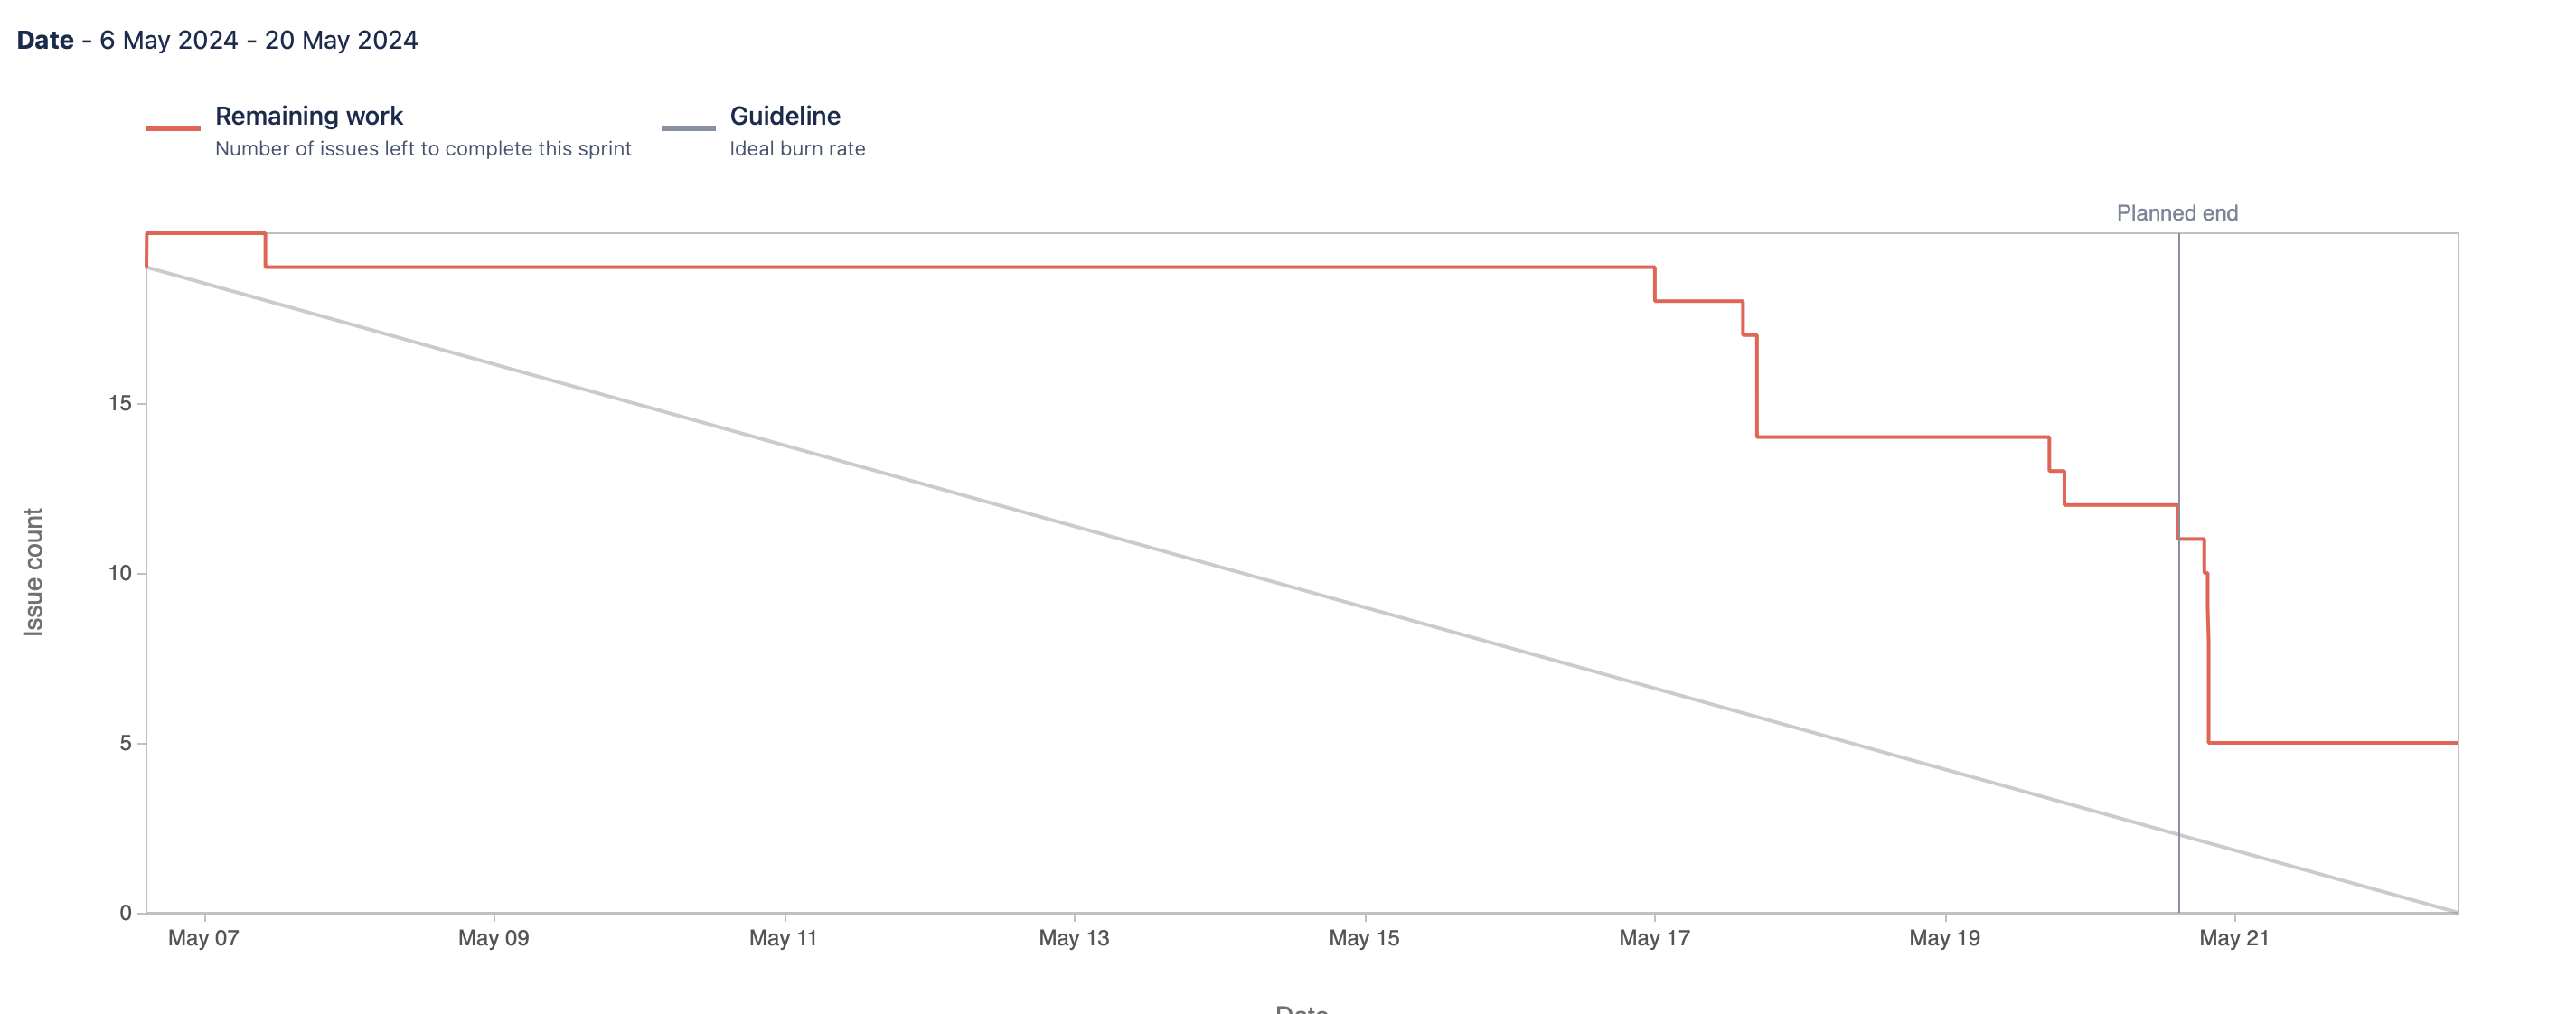
\includegraphics[width=1\textwidth]{Resources/5-Sprint/Review/Burndown.png}
  \caption{Sprint 5 Burndown Chart}
  \label{fig:S5Burndown}
\end{figure}


% Chapter 4
\chapter{Technical Details}
Technical Details Chapter goes here

% Chapter 4a
\section{Design and UML Diagrams}
Design and UML Diagrams yapping goes here

% Chapter 4b
\section{Simple Design}
Simple design yapping goes here

% Chapter 4c
\section{Incremental Design}
Incremental Design yapping goes here

% Chapter 4d
\section{Refactoring}
Refactoring yapping goes here

% Chapter 4e
\section{Test-Driven Development}
Test-Driven Development yapping goes here

% Chapter 4f
\section{Unit Testing}
Unit Testing yapping goes here

% Chapter 4g
\section{Pair Programming}
Pair Programming yapping goes here

% Chapter 4h
\section{Code Review}
Code Review yapping goes here

% Chapter 5
\chapter{Conclusion and Group's Reflections}
Conclusion chapter goes here

% Chapter 5a
\section{Working on a common project with other groups}
5a yapping goes here

% Chapter 5b
\section{What went well and not so well with the group's specific set of tasks}
5b yapping goes here

% Chapter 5c
\section{Specific contributions of each team member}
5c yapping goes here

\section{Future actions to prevent problems and difficulties faced during the project}
5d yapping goes here


\end{document}